% TiMBL 6.3 manual

\documentclass{report}

\usepackage{epsf}
\usepackage{epsfig}
\usepackage{a4wide}
\usepackage{palatino}
\usepackage{fullname}
\usepackage{url}

\newcommand{\chisq}{{$ \chi^2 $}}

\author{Walter Daelemans* \and Jakub Zavrel*$\dagger$ \and Ko van der Sloot \and
	Antal van den Bosch\\ \ \\
	Induction of Linguistic Knowledge Research Group\\
	Tilburg centre for Creative Computing\\
        Tilburg University \\ \\
	(*) CLiPS - Computational Linguistics Group\\
        Department of Linguistics \\
	University of Antwerp\\ \\
	($\dagger$) Textkernel B.V.\\ \\
        P.O. Box 90153, NL-5000 LE, Tilburg, The Netherlands \\ 
        URL: http://ilk.uvt.nl\thanks{This document is available from
	http://ilk.uvt.nl/downloads/pub/papers/ilk.TODO.pdf. All rights reserved
	Induction of Linguistic Knowledge, Tilburg University and 
        CLiPS, University of Antwerp.}}

\title{{\huge TiMBL: Tilburg Memory-Based Learner} \\ \vspace*{0.5cm}
{\bf version 6.3} \\ \vspace*{0.5cm}{\huge Reference Guide}\\
\vspace*{1cm} {\it ILK Technical Report -- ILK TODO}}

%better paragraph indentation
\parindent 0pt
\parskip 9pt

\begin{document}

\pagenumbering{roman} 

\maketitle

\tableofcontents

\chapter*{Preface}

Memory-Based Learning ({\sc mbl}) is an elegantly simple and robust
machine-learning method applicable to a wide range of tasks in Natural
Language Processing (NLP).  In our research group at Tilburg
University, we have been working since the end of the 1980s on the
development of Memory-Based Learning techniques and algorithms. The
foundations are bundled in
\namecite{Daelemans+05}. Section~\ref{furtherreading} provides a
historical overview of work on the application of {\sc mbl} in
NLP. With the establishment of the ILK (Induction of Linguistic
Knowledge) research group in 1997, and with the increasing use of {\sc
  mbl} at the CNTS (now CLiPS) research group of the University of
Antwerp, the need for a well-coded and uniform tool for our main
algorithms became more urgent. TiMBL was the result of combining ideas
from a number of different {\sc mbl} implementations, cleaning up the
interface, and using a whole bag of tricks to make it more
efficient. We think it has become a useful tool for NLP research, and,
for that matter, for many other domains where classification tasks are
learned from examples, so we started to release the software in
1999. With the release of the sixth version of TiMBL we moved to
releasing our software under the GPL license, for anyone to use under
the conditions stated in the license.

Memory-Based Learning is a direct descendant of the classical
$k$-Nearest Neighbor ($k$-NN) approach to classification, which has
become known as a powerful pattern classification algorithm for
numeric data. In typical NLP learning tasks, however, the focus is on
discrete data, very large numbers of examples, and many attributes of
differing relevance. Moreover, classification speed is a critical
issue in any realistic application of Memory-Based Learning. These
constraints demand non-trivial data-structures and speedup
optimizations for the core $k$-NN classifier. Our approach has
resulted in an architecture which compresses the typical flat file
organization found in straightforward $k$-NN implementations, into a
decision-tree structure. While the decision tree can be used to
retrieve the exact $k$-nearest neighbors (as happens in the {\sc ib1}
algorithm within TiMBL), it can also be deterministically traversed as
in a decision-tree classifier (the method adopted by the {\sc igtree}
algorithm). We believe that our optimizations make TiMBL one of the
fastest discrete $k$-NN implementations around.

The main effort in the development and maintenance of this software
was and continues to be invested by Ko van der Sloot. The code started
as a rewrite of {\tt nibl}, a piece of software developed by Peter
Berck from a Common Lisp implementation by Walter Daelemans of {\sc
  ib1-ig}. Some of the index optimizations in TiMBL are due to Jakub
Zavrel. The code has benefited substantially from trial, error and
scrutiny by all past and present members of the ILK and CLiPS
(formerly CNTS) groups in Tilburg and Antwerp. We are furthermore
indebted to Ton Weijters of Eindhoven Technical University for his
inspirational early work on $k$-NN and for his involvements in {\sc
  igtree}.

Our sincere thanks go to the many users of TiMBL who have contributed
to it immensely by giving us feedback and reporting bugs, and to the
two organisations that have supported and enabled its development:
NWO, the Netherlands Organization for Scientific Research, and the
Faculty of Humanities of Tilburg University. NWO funding has spanned
three subsequent periods. From 1997 until 2001 development was part of
the ``Induction of Linguistic Knowledge'' research programme,
partially funded by the Netherlands Organization for Scientific
Research (NWO) and Tilburg University. Between 2001 and 2006 it was
funded as part of the ``Memory Models of Language'' research project
under the NWO {\em Vernieuwingsimpuls}\/ programme, and since 2006 it
is funded as part of the ``Implicit Linguistics'' research project
under the NWO Vici programme.

The current release (version 6.3) succeeds major release 6.2. The most
significant change is, that all {\em server} related stuff is moved to a 
separate TimblServer package.
An elaborate description of the changes from
version 1.0 up to 6.3 can be found in Chapter~\ref{changes}.
Although all new features have been tested for
some time in our research groups, the software may still contain bugs
and inconsistencies in some places. We would appreciate it if you
would send bug reports, ideas about enhancements of the software and
the manual, and any other comments you might have, to {\tt
  Timbl@uvt.nl}.

This reference guide is structured as follows. In
Chapter~\ref{license} you can find the terms of the license according
to which you are allowed to use TiMBL. The subsequent chapter gives
some instructions on how to install the TiMBL package on your
computer. Chapter~\ref{changes} lists the changes that have taken
place up to the current version. Next, Chapter~\ref{tutorial} offers a
quick-start tutorial for readers who want to get to work with TiMBL
right away. The tutorial describes, step-by-step, a case study with a
sample data set (included with the software) representing the
linguistic domain of predicting the diminutive inflection of Dutch
nouns.  Readers who are interested in the theoretical and technical
details of Memory-Based Learning and of this implementation can refer
to Chapter~\ref{algorithms}. Chapter~\ref{reference} provides full
reference to the command line options of TiMBL and supported file
formats.

\chapter{GNU General Public License}
\label{license}
\pagenumbering{arabic} 

TiMBL is free software; you can redistribute it and/or modify it under the terms of the GNU General Public License as published by the Free Software Foundation; either version 3 of the License, or (at your option) any later version.

TiMBL is distributed in the hope that it will be useful, but WITHOUT ANY WARRANTY; without even the implied warranty of MERCHANTABILITY or FITNESS FOR A PARTICULAR PURPOSE.  See the GNU General Public License for more details.

You should have received a copy of the GNU General Public License along with TiMBL.  If not, see $<$http://www.gnu.org/licenses/$>$.

In publication of research that makes use of TiMBL 6.3, a citation should be given of: {\em ``Walter Daelemans, Jakub Zavrel, Ko van der
  Sloot, and Antal van den Bosch (2009). TiMBL: Tilburg Memory Based
  Learner, version 6.3, Reference Guide. ILK Technical Report TODO
  Available from \\ {\tt
    http://ilk.uvt.nl/downloads/pub/papers/ilkTODO.pdf}''}

For information about commercial licenses for TiMBL 6.3,
contact {\tt Timbl@uvt.nl}, or send your request in writing to:

Prof. dr.~Walter Daelemans\\
CLiPS - Language Technology Group\\
Dept. of Linguistics \\
University of Antwerp\\
Prinsstraat 13, L-203, B-2000 Antwerp \\
Belgium

\pagestyle{headings}

\chapter{Installation}
\vspace{-1cm}
You can get the TiMBL package as a gzipped tar archive from:

{\tt http://ilk.uvt.nl/timbl}

Following the links from that page, you can download the file {\tt timbl-6.3.tar.gz}. This file contains the complete source code (C++) for the TiMBL program, a few sample data sets, the license, and documentation. The installation should be relatively straightforward on most UNIX systems.

To install the package on your computer, unzip the downloaded file ({\tt >} is the command line prompt):

{\tt > tar xfz timbl-6.3.tar.gz}

This will make a directory {\tt timbl-6.3} under your current directory.

Alternatively you can do:

{\tt > gunzip timbl-6.3.tar.gz}

and unpack the tar archive:

{\tt > tar xf timbl-6.3.tar}

Go to the timbl-6.3 directory, and configure the package by typing

{\tt > cd timbl-6.3} \\
{\tt > ./configure --prefix=<location\_to\_install>}

If you do not use the {\tt --prefix} option, TiMBL will try to install itself in the directory {\tt /usr/local/}.  If you do not have {\tt root} access you can specify a different installation location such as {\tt \$HOME/install}

It is not obligatory to install TiMBL, but if you plan to install TiMBL-based extensions such as Mbt\footnote{\url{http://ilk.uvt.nl/mbt}}, Dimbl\footnote{\url{http://ilk.uvt.nl/dimbl}}, or Tadpole\footnote{\url{http://ilk.uvt.nl/tadpole}}, or you want to build your own extensions using the TiMBL API, installing is the best choice.

After {\tt configure} you can build TiMBL:

{\tt > make}

and (as recommended) install:

{\tt > make install }

If the process was completed successfully, you should now have executable files
named {\tt Timbl} and {\tt TimblClient} in the directory 
{\tt <location\_to\_install>/bin}, and a static library {\tt libTimbl.a} in the
 directory {\tt <location\_to\_install>/lib}. Additionally, several demo programs named {\tt api\_test*}, {\tt classify} and {\tt tse}
are created in the {\tt ./demos} subdirectory.

Within the {\tt <location\_to\_install>} directory a subdirectory is also created: {\tt share/doc/timbl} where the TiMBL 6.3 documentation can be found, and which in turn contains a subdirectory {\tt examples} with example data files. Some of these data sets are used in the Quick Start Section~\ref{tutorial} of this document; other data and source files are referred to in the API documentation. The latter, along with a pdf version of this document, can also be found in the {\tt doc} directory. Note that the API documentation is a beta-state document.

TiMBL should now be ready for use. If you want to run the examples and demos from this manual, you should act as follows:

\begin{itemize}
\item Be sure to add {\tt <location\_to\_install>/bin} to your PATH. 
In many shells something like

 {\tt > export PATH=\$PATH:<location\_to\_install>/bin }
will do.
\item copy all the files from {\tt
  <location\_to\_install>/share/doc/timbl/examples} to some working
location. (By default, TiMBL writes its results to the directory where
it finds the data.)
\item and test:

{\tt cd} to the working location, and then

{\tt Timbl -f dimin.train -t dimin.test}
\end{itemize}

If you did not install TiMBL, the executable can be found in the {\tt src} directory of the build. The demo files can be found in the {\tt demo} directory.

The e-mail address for problems with the installation, bug reports, comments and questions is {\tt Timbl@uvt.nl}.

\chapter{Changes}
\label{changes}

This chapter gives a brief overview of the changes from all previously released versions (1.0 up to 6.3) for users already familiar with the program.

\section{From version 6.2 to 6.3}

\begin{itemize}
\item All server related functionality is removed from Timbl. A new TimblServer package is available wich provides the same interface as Timbl upto 6.3, but also adds some extra features, like running serveral several unrelated experiments on one TCP port. See the TimblServer package for more details.

\item Starting with Timbl 6.3, we will support installable packages for Debian and Ubuntu (.deb), RedHat (.rmp) and MacOSX (Fink) (see TODO)

\item As usual, some bugs and inconsistencies have been fixed.

\end{itemize}

\section{From version 6.1 to 6.2}

Version 6.2 differs from 6.1 in a great number of internal changes aimed at making the code better maintainable and extendible, in some minor bug fixes, and in the following more prominent changes:

\begin{itemize}

\item A new distance metric, the Dice coefficient, has been added; the metric can be set with {\tt -mDC}. Analogous to the Levenshtein ({\tt -mL}) metric, the Dice coefficient operates at the feature value level; it computes the overlap in character bigrams of two value strings.

\item Value difference matrices, as used by the {\sc mvdm} and Jeffrey divergence distance metrics, can now be written to file, and read into TiMBL, allowing for user-defined value difference metrics to be used. The new command line options are {\tt --matrixout=<filename>} and {\tt --matrixin=<filename>}.

\item The {\sc IGTree} algorithm has been optimized beyond the improvements introduced in version 6.0. With very large training sets, {\sc IGTree} was reported to be exponentially slower in the later stages of training. Trees are now built in near-linear time.

\end{itemize}

Finally, besides minor bug fixes, a great number of internal changes were made to make the code better maintainable and extendible.

\section{From version 6.0 to 6.1}

Version 6.1 differs from 6.0 mainly in the changed configuration.  It is now based on autotools and is delivered as an installable package.  Some bugs have been fixed as well.

\section{From version 5.1 to 6.0}

Version 6.0 differs from 5.1 firstly in terms of internal changes aimed at increasing classification speed and lowering memory usage, of which the most prominent are

\begin{itemize}

\item The {\sc IGTree} algorithm has been optimized. Learning has been
  made more memory-lean, while classification has been optimized so
  that it is now orders of magnitude faster than before on most data sets.

\item {\sc Mvdm} matrices are partly prestored; only the {\sc mvdm}
  values of pairs of frequent values are precomputed. The threshold
  frequency $n$ can now be determined with {\tt -c n}. This way memory
  can be traded for speed, up to a point. The default value 10 remains
  the recommended one.

\end{itemize}

Also, two metrics and several verbosity options and other command-line
switches are added:

\begin{itemize}

\item Two distance metrics are added: {\tt -mC} sets the Cosine
  metric, and {\tt -mL} sets the Levenshtein metric. The latter metric
  operates at the feature-value level, and thus offers an alternative
  to the all-or-nothing Overlap metric for string-valued features. 

\item Class distribution output generated with {\tt +v db} can be
  normalized so that they add to $1.0$, with the additional {\tt -G}
  option (or {\tt -G0}). As a simple smoothing option, with {\tt
    -G1:double} all class votes are incremented by {\tt double} before
  normalization.  For example, {\tt -G1:1} (or {\tt -G1} for short) is
  ``add one''-smoothing; {\tt -G1:0.5} adds $0.5$ to all class votes.

\item With {\tt -Beam=n} (from version 6.2 onwards: {\tt --Beam=n}), where $n$ is an integer, the {\tt +v db}
  output is constrained to the $n$ classes receiving the highest
  votes. This special limit is useful in cases in which the {\tt +v
    db} output, typically used for further processing, generates far
  too much output in its default unconstrained setting. 

\item Class distributions are not stored on non-terminal nodes with
  {\sc IGTree} and {\sc tribl} by default. To revert this default,
  e.g. to be able to use {\tt +v db} with {\sc IGTree}, the setting
  {\tt +D} can be used.

\item With {\tt -T n}, the user can specify that the $n$th column in
  the training set of labeled examples contains the label to be
  predicted, while all other columns represent the input features. By
  default, the last column is assumed to contain the class labels.

\item After classification, TiMBL reports its classification speed at
  microsecond precision instead of in seconds.

\item The verbosity option {\tt +v md} displays the level at which a
  classification was made by {\sc IGTree} ({\tt -a1}), and whether the
  class label was obtained from a leaf node or an end node.

\item With {\tt -X [file]}, TiMBL dumps its internal TiMBL tree into a
  file containing an XML tree. This option is analogous to {\tt -I
    [file]}, which prints a TiMBL tree in TiMBL's proprietary format,
  the difference being that the latter format can be read into TiMBL
  again.

\item Several minor bugs have been resolved.

\end{itemize}

\section{From version 5.0 to 5.1}

Version 5.1 adds speed and memory improvements that are notable with
datasets that have very large amounts of examples, features, feature
values, or classes (and, especially, combinations of those). Previous
versions exhibited exponential slowdown in some worst cases; this has
been largely countered. On the outside, TiMBL has been updated in the
following aspects:

\begin{itemize}

\item TiMBL offers extended performance reporting: next to accuracy it
  reports on micro and macro-averages of F-score and AUC (area under
  the ROC-curve) with {\tt +v as}. Optionally, it also shows each
  individual class' precision, recall (or true positive rate), and
  false positive rate with {\tt +v cs}.

\item TiMBL always uses gain ratio feature weighting as the default
  case, if not specified by the user, also with the {\sc mvdm} and
  Jeffrey Divergence similarity metrics.

\item Two additional feature orderings for the internal TiMBL trees
  are added, {\tt -TGxE} and {\tt -TIxE} (gain ratio $\times$ entropy
  and information gain $\times$ entropy, respectively) to potentially
  tackle the problem of unbalanced trees.

\item Bugs in leave-one-out testing with numeric features and with
  exemplar weighting were fixed.

\end{itemize}

\section{From version 4.3 to 5.0}

Version 5.0 is the conclusion of a number of recodings (mostly
involving more generic treatment of variables to improve robustness,
but also the removal of inverted indexing on the internal tree
representation) that have changed the internals of TiMBL
considerably. On the outside, TiMBL displays the following new
characteristics:

\begin{itemize}

\item Next to the Overlap, {\sc mvdm}, and Numeric distance functions,
  TiMBL now features the Jeffrey divergence distance function and the
  Dot-product distance function.

\item The exponential-decay distance weighting function can be set
  using a second parameter, which can change the shape of the function
  from normal exponential to bell-shaped.

\item In addition to the ``binary'' format, TiMBL can now read
  a more generic sparse data format. This format allows instances to
  be coded by tuples of $<$ feature number, feature value $>$ where the
  value can be symbolic or numeric rather than only binary.

\item Tree files generated by TiMBL versions 1.*, 2.* and 3.* are no
longer supported.

\item The command line interface has had the following additions, including the ones reflecting the above changes:

\begin{itemize} 
\item {\tt -m J} activates the Jeffrey divergence distance metric.
\item {\tt -m D} activates the Dot-product distance metric.
\item {\tt -d ED:<a>:<b>} (without whitespace) sets the $\alpha$ and new
  $\beta$ parameters. If unspecified, as in {\tt -d ED:<a>} or the older
  (deprecated) {\tt -d ED <a>}, $\beta$ is set to $1.0$.
\item {\tt -F Sparse} declares that training and test files are in the
  sparse $<$ feature number, feature value $>$ tuple-format described in
  more detail in section~\ref{commandline}.
\item {\tt +v k} is a new verbosity option that prints all class
distributions per $k$-nearest distance per classified instance in the
output file. It works analogous to the {\tt +v n} option, but does not
print the neighbors themselves.
\end{itemize}

\end{itemize}

\section{From version 3.0 to 4.3}

As the last upgrade of the version 4 strain, version 4.3 added some
command line functionality and internal code changes to version
4.2. Minor progressive changes from 4.0 to 4.3 are found at the bottom
of this list and are marked as such.

\begin{itemize}

\item Distance weighting of the $k$ nearest neighbors. This classical
exemplar weighting scheme \cite{Dudani76} allows closer nearest
neighbors in the $k$ to have a more prominent vote in
classification. TiMBL incorporates linear, inversed, and exponential
distance weighting.

\item Incremental edited memory-based learning with {\sc ib2}
\cite{Aha+91}. This incremental version of {\sc ib1} adds instances to
memory only when those instances are misclassified by the then-current
set of instances in memory.

\item Frequency-filtered {\sc mvdm} distance metric. The option, which is
not selected by default, is an add-on of the {\sc mvdm} metric, that backs
off from the {\sc mvdm} metric to the Overlap distance function whenever one
or both in a pair of matched values occurs fewer times in the training
material than a user-determined threshold.

\item {\sc tribl2}. The {\sc tribl2} algorithm has been implemented
as an additional trade-off between {\sc igtree} and {\sc ib1}. In
contrast to {\sc tribl}, {\sc tribl2} uses no threshold parameter.

\item Exemplar weighting. TiMBL can read additional numeric exemplar
weights (generated externally) when reading a data file, and use these
weights during neighbor distance computation in $k$-NN classification.

\item Cross-validation testing. Analogous to the leave-one-out testing
option, with cross-validation testing it is possible to let TiMBL run
systematic tests on different values of parameters, without completely
re-initializing the classifier in every fold of the validation experiment.

\item The number of concurrent connections to a TiMBL server has been
restricted, but can be set to different values.

\item The command line interface has had several additions reflecting
the above changes, plus one extra verbosity option:

\begin{itemize} 
	\item the {\tt -d metriccode} option sets the distance
          weighting metric. Three metrics are available: inverse
          distance (code ID), inverse linear (IL), and exponential
          decay (ED, which takes an extra argument $a$, without
          whitespace, determining the factor of the exponential
          function). By default, no distance weighting is used (code
          Z). See Chapter~\ref{algorithms} for descriptions.
        \item the {\tt -L n} option sets the frequency threshold in
          the optional switch (backoff) from {\sc mvdm} or Jeffrey
          divergence to Overlap; whenever in an {\sc mvdm} or Jeffrey
          divergence distance computation one or both of a pair of
          values occur fewer than {\tt n} times, Overlap is used
          rather than the {\sc mvdm} metric.  The default value for
          {\tt n} is 1 (no switching).
	\item the {\tt -a 3} or {\tt -a IB2} switch invokes the 
              {\sc ib2} algorithm. This algorithm expects to have 
              the {\tt -b} switch set.
	\item the {\tt -b n} option sets the number ($n$) of lines
              counting from the top of the training set file, which form
              the bootstrap set of memorized instances to which {\sc ib2} 
              will start adding instances incrementally.
	\item the {\tt -a 4} or {\tt -a TRIBL2} switch invokes the 
              {\sc tribl2} algorithm.
        \item the {\tt -C n} switch (default: {\tt n} set to 10) restricts
              the number of concurrent connections to a TiMBL server
              (cf. the {\tt -S} switch).
	\item the {\tt +v/-v} option has {\tt cm} as a new optional
              argument; it returns the confusion matrix, obtained
              after testing, between predicted and actual classes in 
              the test data.
\end{itemize}

\item The ``programmer's reference'' or API section has been separated
  from this manual. This new API, describing the underlying structure
  of TiMBL, is available as a separate document in the TiMBL software
  distribution.

\item Two bugs relating to a type of sparse data problem have been
resolved. The first involved leave-one-out experiments on data sets
with features that have values that occur only once in the training
data. The second bug occurred with the use of the {\tt -F Binary}
option with the same type of data.

\item {\bf [4.1]} Exemplar weights are stored in the TiMBL-tree.

\item {\bf [4.1]} The core representation of
TiMBL-trees has been modified, causing no changes at the surface
except that the {\sc tribl} variant uses less memory.

\item {\bf [4.2]} Feature value and class information in the internal
TiMBL tree is hashed, by default, except with binary features. Hashing
can be explicitly set on or off through the flag {\tt +H} or {\tt -H}.

\item {\bf [4.2]} The discretization of numeric
features, used for computing feature weights, has changed from linear
binning between minimum and maximum values, to equal-content binning.

\item {\bf [4.2]} Tie resolution between equal
class distributions in the nearest neighbors set is resolved by first
expanding the $k$ by one value. If the tie persists after the
enlargement of the nearest neighbor set, the original tie resolution
method is applied.

\item {\bf [4.3]} Internal changes in the code (with no effect on
learning and classification functionality) have been implemented with
respect to namespaces.

\item {\bf [4.3]} A progress marker (one dot per 10 seconds) in
computationally intensive operations on the internal representation of
the instance base (e.g. pruning {\sc igtree}s) is added in TiMBL's
screen output.

\item A number of bugs have been fixed, notably to handle erroneous
input more robustly.

\end{itemize}

\section{From version 2.0 to 3.0}

\begin{itemize}

\item Server functionality. Apart from the standard processing of test
items from a file, alternatively you can now specify a portnumber with
{\tt -S portnumber} to open a socket and send commands for
classification of test patterns or change of parameters to it. A
sample client program is included in the distribution. This allows
fast response times when small amounts of test material are presented
at various intervals. It also opens the possibility of having large
numbers of ``classification agents'' cooperate in real time, or of
classication of the same data with different parameters. The syntax of
our simple Client/Server protocol is described in
Chapter~\ref{serverformat}.

\item Leave-one-out testing. To get an estimate of the classification
error, without setting aside part of one's data as a test set, one
can now test by ``leave-one-out'' ({\tt -t leave\_one\_out}), in effect
testing on every case once, while training on the rest of the cases,
without completely re-initializing the classifier for every test case.

\item Support for sparse binary features. For tasks with large numbers
of sparse binary features, TiMBL now allows for an input format which
lists only the ``active'' features, avoiding the listing of the many
(zero-valued) features for each case. This format is described in
Section~\ref{binaryformat}.

\item Additional feature weighting metrics. We have added chi-squared
and shared variance measures as weighting schemes. These weighting
metrics are sometimes more robust to large numbers of feature values
and other forms of data sparseness.

\item Different metrics (Overlap, {\sc mvdm} or Numeric) can be
applied to different features.

\item The command line interface has slightly been cleaned up, and
re-organized:

\begin{itemize}

\item The {\tt -m metricnumber} switch to choose metrics has been
replaced by the use of a specification string following {\tt
-m}. E.g.~you can specify to use {\sc mvdm} as the default metric, but
use Overlap on features 5-7,9, Numeric on feature 1, and ignore
feature 10 ({\tt -m M:O5-7,9:N1:I10}).

\item All of the output needed for analysing the matching of nearest
neighbors has been moved to the verbosity setting.

\item Verbosity levels and some other options can be switched on {\tt
+v} and off {\tt -v}, even between different classification actions.

\item Because of the large amount of verbosity levels, the {\tt +v}
option takes mnemonic abbreviations as arguments instead of numeric
verbosity levels. Although the old (numeric) format is still
supported, it's use is not encouraged as it will disappear in future
versions.

\end{itemize}

\item Because of significant optimizations in the nearest neighbor
search, the default is no longer to use inverted indexes. These can
however still be turned on by using the {\tt +-} switch on the command
line.

\item You can now choose the output filename or have it generated by
TiMBL on the basis of the test filename and the parameters.

\item You can use TiMBL in a pipeline of commands by specifying '-' as
either input, output or both.

\item Several problems with the display of nearest neighbors in the
output have been fixed.

\item The API has been adapted a bit to allow more practical use of
it.

\end{itemize}

\section{From version 1.0 to 2.0}

\begin{itemize}

\item We have added a new algorithm: {\sc tribl}, a hybrid between
the fast {\sc igtree} algorithm and real nearest neighbor search (for
more details, see~\ref{tribl}, or~\namecite{Daelemans+97d}). This
algorithm is invoked with the {\tt -a 2} switch and requires the
specification of a so-called {\sc tribl}-offset, the feature where
{\sc igtree} stops and case bases are stored under the leaves of the
constructed tree.

\item Support for numeric features. Although the package has retained
its focus on discrete features, it can now also process numeric
features, scale them, and compute feature weights on them. You
specify which features are numeric with the {\tt -N} option on the
command line.

\item The organization of the code is much more object-oriented than
in version 1.0. 
%The main benefit of this is that:

\item A Memory-Based Learning API is made available. You can define
Memory-Based classification objects in your own C++ programs and
access all of the functionality of TiMBL by linking to the TiMBL
library.

\item It has become easier to examine the way decisions are made from
nearest neighbors, because several verbosity-levels allow you to dump
similarity values ({\tt -D}), distributions ({\tt -v 16}), and nearest
neighbor sets ({\tt -v 32}) to the output file. The {\tt -d} option
for writing the distributions no longer exists.

\item Better support for the manipulation of {\sc mvdm}
matrices. Using the {\tt -U} and {\tt -u} options it is now possible
to respectively save and read back value difference matrices (see
Section~\ref{mvdmformat}).

\item Both ``pre-stored'' and ``regular'' {\sc mvdm} experiments now
generate filenames with ``{\tt mvd}'' in the suffix. This used to be
``{\tt pvd}'' and ``{\tt mvd}'' respectively.

\item a number of minor bugs have been fixed.

\end{itemize}


\chapter{Quick-start Tutorial}
\label{tutorial}

This quick-start tutorial is meant to get you started with TiMBL
right away. We discuss how to format the data of a task to serve as
training examples, which choices can be made during the construction
of the classifier, how various choices can be evaluated in terms of
their generalization accuracy, and various other practical issues. The
reader who is interested in more background information on TiMBL
implementation issues and a formal description of Memory-Based
Learning, is advised to read Chapter~\ref{algorithms}.

Memory-Based Learning ({\sc mbl}) is based on the idea that
intelligent behavior can be obtained by analogical reasoning, rather
than by the application of abstract {\em mental rules} as in rule
induction and rule-based processing. In particular, {\sc mbl} is
founded in the hypothesis that the extrapolation of behavior from
stored representations of earlier experience to new situations, based
on the similarity of the old and the new situation, is of key
importance.

{\sc mbl} algorithms take a set of examples (fixed-length patterns of
feature-values and their associated class) as input, and produce a
{\em classifier} which can classify new, previously unseen, input
patterns. Although TiMBL was designed with linguistic classification
tasks in mind, it can in principle be applied to any kind of
classification task with symbolic or numeric features and discrete
(non-continuous) classes for which training data is available. As an
example task for this tutorial we go through the application of TiMBL
to the prediction of Dutch diminutive suffixes. The necessary data
sets are included in the TiMBL distribution, so you can replicate the
examples given below on your own system.

\section{Data}

The operation of TiMBL will be illustrated below by means of a real
natural language processing task: prediction of the diminutive suffix
form in Dutch~\cite{Daelemans+97b}. In Dutch, a noun can receive a
diminutive suffix to indicate {\em small size} literally or
metaphorically attributed to the referent of the noun; e.g. {\em
mannetje} means {\em little man}. Diminutives are formed by a
productive morphological rule which attaches a form of the Germanic
suffix {\em -tje} to the singular base form of a noun. The suffix
shows variation in its form (Table \ref{variation}). The task we
consider here is to predict which suffix form is chosen for previously
unseen nouns on the basis of their form.

\begin{table}[ht]
\begin{center}
\begin{tabular}{l|l|l}
Noun & Form & Suffix \\
\noalign{\smallskip}
\hline
\noalign{\smallskip}
huis (house) & huisje & {\em -je} \\
man (man) & mannetje & {\em -etje\/} \\
raam (window) & raampje & {\em -pje\/} \\
woning (house) & woninkje & {\em -kje\/} \\
baan (job) & baantje & {\em -tje\/} \\
\end{tabular}
\caption{Allomorphic variation in Dutch diminutives.}\label{variation}
\end{center}
\end{table}

For these experiments, we collect a representation of nouns in terms
of their syllable structure as training material\footnote{These words
  were collected form the {\sc celex} lexical
  database~\cite{Baayen+93}.}. For each of the last three syllables of
the noun, four different features are collected: whether the syllable
is stressed or not (values - or +), the string of consonants before
the vocalic part of the syllable (i.e. its onset), its vocalic part
(nucleus), and its post-vocalic part (coda). Whenever a feature value
is not present (e.g. a syllable does not have an onset, or the noun
has less than three syllables), the value `=' is used. The class to be
predicted is either E ({\em -etje}), T ({\em -tje}), J ({\em -je}), K
({\em -kje}), or P ({\em -pje}).

Some examples are given below (the word in the rightmost column is only provided for
convenience and is not used). The values of the syllabic content
features are given in phonetic notation.

\begin{table}[ht]
\begin{center}
\begin{tabular}{cccccccccccc|l|l|l}
+ & b & i & = & - & z & @ & = & - & m & A & nt & J & {\em biezenmand} \\
= & = & = & = & = & = & = & = & + & b & I & x & E & {\em big}\\
= & = & = & = & + & b & K & = & - & b & a & n & T & {\em bijbaan}\\
= & = & = & = & + & b & K & = & - & b & @ & l & T & {\em bijbel}\\
\end{tabular}
\end{center}
\end{table}

Our goal is to use TiMBL in order to train a classifier that can
predict the class of new, previously unseen words as correctly as
possible, given a set of training examples that are described by the
features given above. Because the basis of classification in TiMBL is
the storage of all training examples in memory, a test of the
classifier's accuracy must be done on a separate test set. We will
call these datasets {\tt dimin.train} and {\tt dimin.test},
respectively. The training set {\tt dimin.train} contains 2999 words
and the test set contains 950 words, none of which are present in the
training set. Although a single train/test partition suffices here for
the purposes of explanation, it does not factor out the bias of
choosing this particular split. Unless the test set is sufficiently
large, a more reliable generalization accuracy measurement is used in
real experiments, e.g.~10-fold cross-validation~\cite{Weiss+91}. This
means that 10 separate experiments are performed, and in each ``fold''
90\% of the data is used for training and 10\% for testing, in such a
way that each instance is used as a test item exactly once. Another
reliable way of testing the real error of a classifier is
leave-one-out~\cite{Weiss+91}. In this approach, every data item in
turn is selected once as a test item, and the classifier is trained on
all remaining items. Accuracy of the classifier is then the number of
data items correctly predicted. With the option {\tt -t
leave\_one\_out}, this testing methodology is used by TiMBL. We
will use this option in the tutorial on the file {\tt dimin.data}, the
union of {\tt dimin.train} and {\tt dimin.test}. 

\section{Using TiMBL}

Different formats are allowed for training and test data files. TiMBL
is able to guess the type of format in most cases. We will use
comma-separated values here, with the class as the last value. This
format is called C4.5 format in TiMBL because it is the same as that
used in Quinlan's well-known C4.5 program for induction of decision
trees~\cite{Quinlan93}. See Section~\ref{fileformats} for more
information about this and other file formats.

An experiment is started by executing TiMBL with the two files ({\tt
  dimin.train} and {\tt dimin.test}) as arguments (``$>$'' is the
command line prompt):

{\footnotesize
\begin{verbatim}
> Timbl -f dimin.train -t dimin.test
\end{verbatim}
}

Upon completion, a new file has been created with name {\small\tt
dimin.test.IB1.O.gr.k1.out}, which is identical to the
input test file except that an extra comma-separated column is added
with the class predicted by TiMBL. The name of the file provides
information about the {\sc mbl} algorithms and metrics used in the
experiment (the default values in this case). We will describe these
shortly.

Apart from the result file, information about the operation of the
algorithm is also sent to the standard output. It is therefore 
advisable to redirect the output to a file in order to make a log of
the results.

{\footnotesize
\begin{verbatim}
> Timbl -f dimin.train -t dimin.test > dimin-exp1
\end{verbatim}
}

The defaults used in this case work reasonably well for most problems.  We
will now provide a point by point explanation of what goes on in the
output.

%\vspace{0.5cm}

%\rule{\textwidth}{0.5mm}

{\footnotesize
\begin{verbatim}
TiMBL 6.2.0 (c) ILK 1998 - 2009.
Tilburg Memory Based Learner
Induction of Linguistic Knowledge Research Group, Tilburg University
CLiPS Computational Linguistics Group, University of Antwerp
Mon Oct 19 21:30:00 2009

Examine datafile 'dimin.train' gave the following results:
Number of Features: 12
InputFormat       : C4.5
\end{verbatim}
}

%\rule{\textwidth}{0.5mm}

%\vspace{0.5cm}

TiMBL has detected 12 features and the C4.5 input format
(comma-separated features, class at the end).

%\rule{\textwidth}{0.5mm}

{\footnotesize
\begin{verbatim}
Phase 1: Reading Datafile: dimin.train
Start:          0 @ Mon Oct 19 21:30:00 2009
Finished:    2999 @ Mon Oct 19 21:30:00 2009
Calculating Entropy         Mon Oct 19 21:30:00 2009
Lines of data     : 2999
DB Entropy        : 1.6178929
Number of Classes : 5

Feats	Vals	InfoGain	GainRatio
    1      3	0.030971064	0.024891536
    2     50	0.060860038	0.027552191
    3     19	0.039562857	0.018676787
    4     37	0.052541227	0.052620750
    5      3	0.074523225	0.047699231
    6     61	0.10604433	0.024471911
    7     20	0.12348668	0.034953203
    8     69	0.097198760	0.043983864
    9      2	0.045752381	0.046816705
   10     64	0.21388759	0.042844587
   11     18	0.66970458	0.18507018
   12     43	1.2780762	0.32537181

Feature Permutation based on GainRatio/Values :
< 9, 5, 11, 1, 12, 7, 4, 3, 10, 8, 2, 6 >
\end{verbatim}
}

%\rule{\textwidth}{0.5mm}

%\vspace{0.5cm}

Phase 1 is the training data analysis phase. Time stamps for start and
end of analysis are provided. Some preliminary analysis of the
training data is done: number of training items, number of classes,
entropy of the training data. For each feature, the number of values,
and four variants of an information-theoretic measure of feature
relevance are given. These are used both for memory organization
during training and for feature relevance weighting during testing
(see Chapter~\ref{algorithms}). Finally, an ordering (permutation) of
the features is given. This ordering is used for building the
tree-index to the case-base.

%\vspace{0.5cm}

%\rule{\textwidth}{0.5mm}


{\footnotesize
\begin{verbatim}
Phase 2: Learning from Datafile: dimin.train
Start:          0 @ Mon Oct 19 21:30:00 2009
Finished:    2999 @ Mon Oct 19 21:30:00 2009

Size of InstanceBase = 19231 Nodes, (769240 bytes), 49.77 % compression
Examine datafile 'dimin.test' gave the following results:
Number of Features: 12
InputFormat       : C4.5
\end{verbatim}
}

%\rule{\textwidth}{0.5mm}

%\vspace{0.5cm}

Phase 2 is the learning phase: all training items are stored in an
efficient way in memory for use during testing. Again timing
information (real time) is provided, as well as information about the
size of the data structure representing the stored examples and the
amount of compression achieved. 

%\vspace{0.5cm}

%\rule{\textwidth}{0.5mm}

{\footnotesize
\begin{verbatim}
Starting to test, Testfile: dimin.test
Writing output in:          dimin.test.IB1.O.gr.k1.out
Algorithm     : IB1
Global metric : Overlap
Deviant Feature Metrics:(none)
Weighting     : GainRatio
Feature 1	 : 0.024891535617620
Feature 2	 : 0.027552191321752
Feature 3	 : 0.018676787182524
Feature 4	 : 0.052620750282779
Feature 5	 : 0.047699230752236
Feature 6	 : 0.024471910753751
Feature 7	 : 0.034953203413051
Feature 8	 : 0.043983864437713
Feature 9	 : 0.046816704745507
Feature 10	 : 0.042844587034556
Feature 11	 : 0.185070180760327
Feature 12	 : 0.325371814230901

Tested:      1 @ Mon Oct 19 21:30:00 2009
Tested:      2 @ Mon Oct 19 21:30:00 2009
Tested:      3 @ Mon Oct 19 21:30:00 2009
Tested:      4 @ Mon Oct 19 21:30:00 2009
Tested:      5 @ Mon Oct 19 21:30:00 2009
Tested:      6 @ Mon Oct 19 21:30:00 2009
Tested:      7 @ Mon Oct 19 21:30:00 2009
Tested:      8 @ Mon Oct 19 21:30:00 2009
Tested:      9 @ Mon Oct 19 21:30:00 2009
Tested:     10 @ Mon Oct 19 21:30:00 2009
Tested:    100 @ Mon Oct 19 21:30:00 2009
Ready:     950 @ Mon Oct 19 21:30:00 2009
Seconds taken: 0.0650 (14609.99 p/s)

overall accuracy:        0.968421  (920/950), of which 39 exact matches 
There were 5 ties of which 5 (100.00%) were correctly resolved
\end{verbatim}
}

%\rule{\textwidth}{0.5mm}

%\vspace{0.5cm}

In Phase 3, the trained classifier is applied to the test set. Because
we have not specified which algorithm to use, the default settings are
used ({\sc ib1} with information-theoretic feature weighting). This
algorithm computes the similarity between a test item and each
training item in terms of {\em weighted overlap}: the total difference
between two patterns is the sum of the relevance weights of those
features which are not equal. The class for the test item is decided
on the basis of the least distant item(s) in memory. To compute
relevance, Gain Ratio is used (an information-theoretic measure, see
Section~\ref{infogain}). Time stamps indicate the progress of the
testing phase. Finally, accuracy on the test set is logged, and the
number of exact matches\footnote{An exact match in this experiment can
  occur when two different nouns have the same feature-value
  representation.} and ties (two or more classes are equally frequent
in the nearest neighbor set). In this experiment, the diminutive
suffix form of 96.8\% of the new words was correctly predicted. Train
and test set overlap in 39 items, and the algorithm had to break five
ties, all of which were broken correctly.

The meaning of the output file names can be explained now:\\ {\tt
dimin.test.IB1.O.gr.k1.out} means output file ({\tt .out}) for {\tt
dimin.test} with algorithm {\sc mbl} (={\sc ib1}), similarity computed
as {\em weighted overlap} ({\tt .O}), relevance weights computed with
{\em gain ratio} ({\tt .gr}), and number of most similar memory
patterns on which the output class was based equal to 1 ({\tt .k1}).

\section{Algorithms and metrics}

A precise discussion of the different algorithms and metrics
implemented in TiMBL is given in Chapter~\ref{algorithms}. We will
discuss the effect of the most important ones on our data set.

A first choice in algorithms is between using {\sc ib1} and {\sc
igtree}. In the trade-off between generalization accuracy and
efficiency, {\sc ib1} usually, but not always, leads to more accuracy
at the cost of more memory and slower computation, whereas {\sc
igtree} is a fast heuristic approximation of {\sc ib1}, but sometimes
less accurate. The {\sc igtree} algorithm is used when {\tt -a 1} is
given on the command line, whereas the {\sc ib1} algorithm used above
(the default) would have been specified explicitly by {\tt -a 0}. 

{\footnotesize
\begin{verbatim}
> Timbl -a1 -f dimin.train -t dimin.test
\end{verbatim}} 

We see that {\sc igtree} performs only slightly worse (96.6\%) than
{\sc ib1} (96.8\%) for this train-test partitioning of the data --- it
uses less memory and is faster, however.

When using the {\sc ib1} algorithm, there is a choice of metrics for
influencing the definition of similarity. With {\em weighted overlap},
each feature is assigned a weight, determining its relevance in
solving the task. With the {\em modified value difference metric}
({\sc mvdm}), each pair of values of a particular feature is assigned
a value difference. The intuition here is that in our diminutive
problem, for example, the codas $n$ and $m$ should be regarded as
being more similar than $n$ and $p$. These pair-wise differences are
computed for each pair of values in each feature (see
Section~\ref{mvdm}). Selection between weighted overlap and {\sc mvdm}
is done by means of the {\tt -mM} parameter. The following selects {\sc
mvdm}, whereas {\tt -mO} ({\em weighted overlap}) is the default.

{\footnotesize
\begin{verbatim}
> Timbl -mM -f dimin.train -t dimin.test
\end{verbatim}
}

Especially when using {\sc mvdm}, but also in other cases, it may be
useful to extrapolate not just from the most similar example in
memory, which is the default, but from several. This can be achieved
by using the $-k$ parameter followed by the wanted number of nearest
neighbors. E.g., the following applies {\sc ib1} with the {\sc mvdm}
metric, with extrapolation from the 5 nearest neighbors.

{\footnotesize
\begin{verbatim}
> Timbl -mM -k5 -f dimin.train -t dimin.test
\end{verbatim}
}

Whenever more than one nearest neighbor is taken into account for
extrapolation, it may be useful to weigh the influence of the
neighbors on the final decision as a function of their distance from
the test item. Several possible implementations of this distance
function are provided. E.g., the following provides inverse distance: 

{\footnotesize
\begin{verbatim}
> Timbl -mM -k5 -dID -f dimin.train -t dimin.test
\end{verbatim}
}

Within the {\sc ib1} {\em weighted overlap}\/ option, the default
feature weighting method is gain ratio. Other feature relevance
weighting methods are available as well.  By setting the parameter
{\tt -w} to 0, an {\em unweighted overlap}\/ definition of similarity is created
where each feature is considered equally relevant. In that case, similarity reduces
to the number of equal values in the same position in the
two patterns being compared. As an alternative weighting, users can
provide their own weights by using the {\tt -w} parameter with a
filename in which the feature weights are stored (see
Section~\ref{weightformat} for a description of the format of the
weights file).

\begin{table}
\begin{center}
\begin{tabular}{l|rrrr}
             & no weight & gain  & information & chi    \\
             & (overlap) & ratio & gain        & squared \\
\noalign{\smallskip}
\hline
\noalign{\smallskip}
Overlap,  $-k1$ & 86.4 & 96.8 & 96.7 & 96.7 \\
Overlap,  $-k3$ & 73.1 & 96.4 & 96.8 & 96.9 \\
Overlap,  $-k5$ & 62.6 & 95.4 & 96.1 & 96.1 \\
\hline
\noalign{\smallskip}
{\sc mvdm}, $-k1$ & 95.8 & 96.4 & 96.2 & 96.3 \\
{\sc mvdm}, $-k3$ & 97.3 & 97.6 & 97.6 & 97.6 \\
{\sc mvdm}, $-k5$ & {\bf 97.8} & 97.7 & 97.7 & 97.7 \\
\hline
\noalign{\smallskip}
\end{tabular}
\caption{Some results for diminutive prediction.}
\label{diminresults}
\end{center}
\end{table}

Table \ref{diminresults} shows a small matrix indicating the effect of distance metric (Overlap versus {\sc mvdm}) and weighting method choice on generalization accuracy, using the same training and test set as before, and increasing $k$ from 1 to 3 and 5. While increasing $k$ leads to a deterioration of generalization accuracy with the Overlap function, it leads to improvements with {\sc mvdm}. Another clear contrast is that the absence of feature weighting leads to the lowest scores with the Overlap function, and the highest score with {\sc mvdm} and $k=5$. Given that TiMBL offers several more hyperparameters than only $k$, the distance metric, and the feature weighting metric, it should be obvious that even with a single training and test set experiment, a large experimental matrix can be explored. Unfortunately, the location of the cell with the highest number in this matrix cannot be predicted upfront. It is therefore useful to try out a large set of reasonable combinations of options by cross-validation on the training data to achieve best results with {\sc mbl} \cite{VandenBosch04b}. The option {\tt
  -t @f} where {\tt f} is the name of a file, allows you to predefine various combinations of options to be tested and test them without having the training stages repeated each time. See Chapter \ref{commandline}.

\section{More options}

Several input and output options exist to make life easier while
experimenting. See Chapter~\ref{commandline} for a detailed
description of these options. One especially useful option for testing
linguistic hypotheses is the ignore option, which allows you to skip
certain features when computing similarity. E.g. if we want to test
the hypothesis that only the rime (nucleus and coda) and the stress of
the last syllable are actually relevant in determining the form of the
diminutive suffix, we can execute the following with the previously
best parameter settings to disregard all but the fourth-last and the
last two features. As a result we get an accuracy of
97.1\%.

{\footnotesize
\begin{verbatim}
> Timbl -mM:I1-8,10 -k5 -w0 -f dimin.train -t dimin.test
\end{verbatim}
}

The {\tt +/-v} (verbosity) option allows you to control the amount of
information that is generated in the output, ranging from nearly nothing
({\tt +v s}) to a lot ({\tt +v as+cs+di+db+n+k}). Specific
verbosity settings exist for dumping option settings ({\tt +v o}),
feature relevance weights (default), value-class conditional
probabilities ({\tt +v p}), exact matches ({\tt +v e}), distributions
({\tt +v db}), a confusion matrix ({\tt +v cm}), advanced statistics
besides accuracy: micro-average and macro-average F-score and AUC
({\tt +v as}), per-class advanced statistics ({\tt +v cs}), the
nearest neighbors on which decision are based ({\tt +v n}), just the
class distributions per $k$-nearest distance per classified instance
({\tt +v k}), or the distances to the nearest neighbor ({\tt +v
  di}). E.g. the following command results in an output file with
distributions.

{\footnotesize
\begin{verbatim}
> Timbl +v db -f dimin.train -t dimin.test
\end{verbatim}
}

The resulting output file {\tt dimin.test.IB1.O.gr.k1.out} contains
lines like the following.

{\footnotesize
\begin{verbatim}
+,t,L,=,-,m,@,=,-,l,I,N,E,E { E 1.00000 }
=,=,=,=,=,=,=,=,+,pr,O,p,J,J { E 3.00000, J 12.0000 }
=,=,=,=,=,=,=,=,+,w,e,t,J,J { J 2.00000 }
=,=,=,=,+,t,L,n,-,h,L,s,J,J { J 1.00000 }
=,=,=,=,=,=,=,=,+,t,L,n,T,T { T 1.00000 }
=,=,=,=,=,=,=,=,+,z,o,m,P,P { P 3.00000 }
+,d,a,=,-,m,@,s,-,kr,A,ns,J,J { J 1.00000 }
=,=,=,=,+,=,a,rd,-,m,A,n,E,E { E 2.00000 }
=,=,=,=,=,=,=,=,+,f,M,n,T,T { T 43.0000, E 20.0000 }
-,d,u,=,-,k,@,=,-,m,A,nt,J,J { J 1.00000 }
\end{verbatim}
}

This information can e.g. be used to assign a certainty to a decision
of the classifier, or to make available a second-best back-off option. Another verbosity option, {\tt +v di}, displays the distance to the nearest neighbor:

{\footnotesize
\begin{verbatim}
> Timbl +v di -f dimin.train -t dimin.test

+,l,a,=,-,d,@,=,-,k,A,st,J,J        0.070701
-,s,i,=,-,f,E,r,-,st,O,k,J,J        0.000000
=,=,=,=,=,=,=,=,+,sp,a,n,T,T        0.042845
=,=,=,=,=,=,=,=,+,st,o,t,J,J        0.042845
=,=,=,=,+,sp,a,r,-,b,u,k,J,J        0.024472
+,h,I,N,-,k,@,l,-,bl,O,k,J,J        0.147489
-,m,e,=,-,d,A,l,+,j,O,n,E,E         0.182421
-,sn,u,=,-,p,@,=,+,r,K,=,T,T        0.046229
=,=,=,=,=,=,=,=,+,sp,A,N,E,E        0.042845
+,k,a,=,-,k,@,=,-,n,E,st,J,J        0.114685        
\end{verbatim}
}

This can be used to study how very similar instances (low distance) and
less similar patterns (higher distance) are used in the process of
generalization.

The listing of nearest neighbors is useful for the analysis of the
behavior of a classifier. It can be used to interpret why particular
decisions or errors occur.

{\footnotesize
\begin{verbatim}
> Timbl +v n+k -mM -k3 -w0 -f dimin.train -t dimin.test

+,m,I,=,-,d,A,G,-,d,},t,J,J { J 3.00000 }
# k=1, 1 Neighbor(s) at distance:       0.99179269134432
#       +,p,a,=,-,t,@,rs,-,f,A,t,{ J 1.00000 }
# k=2, 1 Neighbor(s) at distance:       0.99458957262696
#       +,h,o,=,-,n,@,G,-,b,A,k,{ J 1.00000 }
# k=3, 1 Neighbor(s) at distance:       1.0088291749842
#       +,h,E,r,-,d,@,rs,-,t,A,s,{ J 1.00000 }
-,t,@,=,-,l,|,=,-,G,@,n,T,T { T 3.00000 }
# k=1, 1 Neighbor(s) at distance:       0.33024081383366
#       -,x,@,=,+,h,|,=,-,G,@,n,{ T 1.00000 }
# k=2, 1 Neighbor(s) at distance:       0.49144604610567
#       -,d,@,r,-,w,a,=,-,G,@,n,{ T 1.00000 }
# k=3, 1 Neighbor(s) at distance:       0.56944572926932
#       -,st,@,=,-,l,I,=,-,N,@,=,{ T 1.00000 }
\end{verbatim}
}

A confusion matrix, printed when the {\tt +v cm} option is selected,
can bring to light specific errors of the classifier that would not be
apparent from the overall accuracy. Applied to the diminutive data,
the following confusion matrix is computed and printed:

{\footnotesize
\begin{verbatim}
> Timbl +v cm -f dimin.train -t dimin.test

Confusion Matrix:
             T      E      J      P      K 
        -----------------------------------
     T |    453      0      2      0      0 
     E |      0     87      4      1      8 
     J |      1      4    347      0      0 
     P |      0      3      0     24      0 
     K |      0      7      0      0      9 
   -*- |      0      0      0      0      0 

\end{verbatim}
}

The confusion matrix associates the class predicted by TiMBL
(vertically) with the real class of the test items given
(horizontally). All cells outside the diagonal contain errors of one
class being mistaken for another. For example, the K class ({\em
  -kje}) is mispredicted seven times as class E ({\em -etje}).

(The bottom line, labeled with {\tt -*-}, would contain aggregate
counts of classes occuring in the test data that did not occur in the
training data. In the diminutive data this does not occur.)

In general, a confusion matrix allows a more fine-grained analysis of
experimental results and better experimental designs (some parameter
settings may work for some classes but not for others, or some may
improve recall, and others precision, e.g.). From such a matrix, not
only accuracy can be derived, but also a number of additional metrics
that have become popular in machine learning, information retrieval,
and subsequently also in computational linguistics: {\em recall},
{\em precision}, and their harmonic mean {\em F-score}, as well as {\em true
  positive rate}, {\em false positive rate}, and their joint measure
{\em AUC} in ROC space.  The details of these advanced statistics are
given in Section~\ref{advancedstats}.

They can be reported by TiMBL using the {\tt +v as} and {\tt +v cs}
verbosity options:

{\footnotesize
\begin{verbatim}
> Timbl +v as+cs -f dimin.train -t dimin.test

Scores per Value Class:
class |     TP    FP    TN    FN	precision	recall(TPR)	FPR		F-score		AUC
    T |    453     1   494     2 	0.99780 	0.99560 	0.00202 	0.99670 	0.99679
    E |     87    14   836    13 	0.86139 	0.87000 	0.01647 	0.86567 	0.92676
    J |    347     6   592     5 	0.98300 	0.98580 	0.01003 	0.98440 	0.98788
    P |     24     1   922     3 	0.96000 	0.88889 	0.00108 	0.92308 	0.94390
    K |      9     8   926     7 	0.52941 	0.56250 	0.00857 	0.54545 	0.77697
F-Score beta=1, microav: 0.968123
F-Score beta=1, macroav: 0.863060
AUC, microav:            0.980729
AUC, macroav:            0.926462
overall accuracy:        0.968421  (920/950), of which 39 exact matches 
There were 5 ties of which 5 (100.00%) were correctly resolved
\end{verbatim}
}

We hope that this tutorial has made it clear that, once you have coded
your data in fixed-length feature-value patterns, it should be
relatively straightforward to get the first results using TiMBL. You
can then experiment with different metrics and algorithms to try and
further improve your results.

\chapter{Memory-based learning algorithms}
\label{algorithms}

TiMBL is a program implementing several memory-based learning
algorithms. All implemented algorithms have in common that they store some
representation of the training set explicitly in memory. During
testing, new cases are classified by extrapolation from the most
similar stored cases. The main differences among the algorithms
incorporated in TiMBL lie in:

\begin{itemize}
\item The definition of {\em similarity},
\item The way the instances are stored in memory, and
\item The way the search through memory is conducted.
\end{itemize}

In this chapter, various choices for these issues are described. We
start in Section~\ref{mbl} with a formal description of the basic
memory-based learning algorithm, i.e.~a nearest neighbor search. We
then introduce different distance metrics, such as Information Gain
weighting, which allows us to deal with features of differing
importance, and the Modified Value Difference metric, which allows us
to make a graded guess of the match between two different symbolic
values, and describe the standard versus three distance-weighted
versions of the class voting mechanism of the nearest neighbor
classifier. In Section~\ref{indexing}, we give a description of
various algorithmic optimizations for nearest neighbor search.

Sections~\ref{igtree} to~\ref{ib2} describe three variants of the
standard nearest neighbor classifier implemented within TiMBL, that
optimize some intrinsic property of the standard algorithm. First, in
Section~\ref{igtree}, we describe {\sc igtree}, which replaces the
exact nearest neighbor search with a very fast heuristic that exploits
the difference in importance between features. Second, in
Section~\ref{tribl}, we describe the {\sc tribl} algorithm, which is a
hybrid between {\sc igtree} and nearest neighbor search. Third,
Section~\ref{ib2} describes the {\sc ib2} algorithm, which
incrementally and selectively adds instances to memory during
learning.

The chapter is concluded by Section~\ref{furtherreading}, which
provides an overview of further reading into theory and applications
of memory-based learning to natural language processing tasks.

\section{Memory-based learning}
\label{mbl}

Memory-based learning is founded on the hypothesis that performance in
cognitive tasks is based on reasoning on the basis of similarity of
new situations to {\em stored representations of earlier experiences},
rather than on the application of {\em mental rules}\/ abstracted from
earlier experiences (as in rule induction and rule-based processing).
The approach has surfaced in different contexts using a variety of
alternative names such as similarity-based, example-based,
exemplar-based, analogical, case-based, in\-stance-based, and lazy
learning~\cite{Stanfill+86,Aha+91,Cost+93,Kolodner93,Aha97a}.
Historically, memory-based learning algorithms are descendants of the
$k$-nearest neighbor (henceforth $k$-{\sc nn}) algorithm
\cite{Cover+67,Devijver+82,Aha+91}.

An {\sc mbl} system, visualized schematically in
Figure~\ref{mbl-method}, contains two components: a {\em learning
component}\/ which is memory-based (from which {\sc mbl} borrows its
name), and a {\em performance component}\/ which is similarity-based.

The learning component of {\sc mbl} is memory-based as it involves
adding training instances to memory (the {\em instance base} or case
base); it is sometimes referred to as `lazy' as memory storage is done
without abstraction or restructuring.  An instance consists of a
fixed-length vector of $n$ feature-value pairs, and an information
field containing the classification of that particular feature-value
vector.  

In the performance component of an {\sc mbl} system, the product of
the learning component is used as a basis for mapping input to output;
this usually takes the form of performing classification.  During
classification, a previously unseen test example is presented to the
system. The similarity between the new instance $X$ and all examples
$Y$ in memory is computed using some {\em distance metric}
$\Delta(X,Y)$. The extrapolation is done by assigning the most
frequent category within the found set of most similar example(s) (the
$k$-nearest neighbors) as the category of the new test example. In
case of a tie among categories, a tie breaking resolution method is
used. This method is described in subsection~\ref{tiebreaking}.

\begin{figure}[htb]
        \begin{center}
                \leavevmode
                \epsfxsize=8cm
                \epsffile{mble-method.eps}
                \caption{General architecture of an {\sc mbl} system.
                }
                \label{mbl-method}
        \end{center}
\end{figure}

\subsection{The Overlap metric}
\label{overlap}

The most basic metric that works for patterns with symbolic features
is the {\bf Overlap metric}\footnote{This metric is also referred to
as Hamming distance, Manhattan metric, city-block distance, or L1
metric.} given in Equations~\ref{distance} and~\ref{overlapeq}; where
$\Delta(X,Y)$ is the distance between instances $X$ and $Y$,
represented by $n$ features, and $\delta$ is the distance per
feature. The distance between two patterns is simply the sum of the
differences between the features. The $k$-{\sc nn} algorithm with this
metric is called {\sc ib1} \cite{Aha+91}. 

\begin{equation}
\Delta(X,Y) = \sum_{i=1}^{n} \delta(x_{i},y_{i})
\label{distance}
\end{equation}

where:
\begin{equation}
\delta(x_{i}, y_{i}) = \left\{ \begin{array}{ll}
		abs(\frac{x_{i}-y_{i}}{max_{i}-min_{i}}) & \mbox{if numeric, else}\\
		0 & \mbox{if $x_{i} = y_{i}$}\\
		1 & \mbox{if $x_{i} \neq y_{i}$}\\
	\end{array} \right.
\label{overlapeq}
\end{equation}

The major difference with the {\sc ib1} algorithm originally proposed
by \cite{Aha+91}, is that in our version the value of $k$ refers to
$k$-nearest {\em distances}\/ rather than $k$-nearest examples. With
$k=1$, for instance, TiMBL's nearest neighbor set can contain several
instances that are equally distant to the test instance. Arguably, our
$k$-NN kernel could therefore be called $k$-nearest distances
classification.

Another difference with the original {\sc ib1} as well as with other
implementations such as $k$-NN in the {\sc weka} machine learning
toolkit \cite{Witten+99} is the way in which ties are resolved in
choosing the majority category among the set of nearest
neighbors. Since this method is independent of the distance function
we discuss this issue separately in subsection~\ref{tiebreaking}.

\paragraph{Variations on Overlap: Levenshtein and Dice coefficient metrics}

The Overlap metric is all-or-nothing. For measuring the similarity
between numeric or atomically symbolic values this may suffice, but
there are cases (such as in natural language processing) in which
string-valued feature values occur that can mismatch with other string
values in a meaningfully graded way. For example, the value pair
``bathe'' and ``bathes'' only differs in one letter; counting them as
more similar than ``bathe'' and ``rumour'', for example, may be useful
for the classification task at hand. We implemented two additional
metrics, Levenshtein distance and the Dice coefficient, that each
provide a graded similarity score between pairs of strings.

{\bf Levenshtein} distance is a classic {\em edit distance}\/ metric
\cite{Levenshtein66} that counts the number of insertions, deletions,
and substitutions to transform the one string into the other. In our
(dynamic programming) implementation the three operations count
equally heavily. The {\bf Dice} coefficient computes the overlap
between the occurrences of character bigrams in two strings as in
Equation~\ref{dice}, where $n_{x_{i} \cap y{i}}$ is the number of
character bigrams (uniquely) occuring both in string value $x_{i}$ and
in string value $y_{i}$ (and where $i$ is the index of the feature as
introduced in Equation~\ref{distance})\footnote{Strings of length one
  are not handled by Dice; we back off to Overlap in these
  cases.}. The equation subtracts the similarity from 1, because we
assume $\delta$ to produce a distance, not a similarity.

\begin{equation}
\delta(x_{i}, y_{i}) = 1 - \frac{2 n_{x_{i} \cap y_{i}}}{n_{x_{i}} + n_{y_{i}}}
\label{dice}
\end{equation}

\subsection{Information-gain and gain ratio feature weighting}
\label{infogain}

The distance metric in Equation~\ref{overlapeq} straightforwardly counts the
number of (mis)matching feature-values in both patterns. In the
absence of information about feature relevance, this is a reasonable
choice. Otherwise, we can add domain knowledge bias to weight or
select different features (see e.g.~\namecite{Cardie96} for an
application of linguistic bias in a language processing task), or look
at the behavior of features in the set of examples used for
training. We can compute statistics about the relevance of features by
looking at which features are good predictors of the class
labels. Information Theory gives us a useful tool for measuring
feature relevance in this way~\cite{Quinlan86,Quinlan93}.

{\bf Information Gain} (IG) weighting looks at each feature in
isolation, and measures how much information it contributes to our
knowledge of the correct class label. The Information Gain of feature
$i$ is measured by computing the difference in uncertainty
(i.e.\ entropy) between the situations without and with knowledge of
the value of that feature (Equation~\ref{IGgain}).

\begin{equation}
w_{i} = H(C) -  \sum_{v \in V_{i}} P(v) \times H(C|v)
\label{IGgain}
\end{equation}

Where $C$ is the set of class labels, $H(C) = - \sum_{c \in C} P(c) \log_{2} P(c)$ is the entropy of the class labels, and $V_{i}$ is the set of values for feature $i$. The probabilities are estimated from relative frequencies in the training set.

For numeric features, an intermediate step needs to be taken to apply
the symbol-based computation of IG. All real values of a numeric
features are temporarily discretized into a number (the default is 20)
of intervals. Instances are ranked on their real value, and then
spread evenly over the intervals; each interval contains the same
number of instances (i.e., by default, $1/20$th of the total amount of
instances). Instances in each of these intervals are then used in the
IG computation as all having the same unordered, symbolic value per
group. Note again that this discretization is only temporary; it is
not used in the computation of the distance metric.

It is important to realize that the IG weight is really a
probability-weighted average of the informativity of the different
values of the feature. On the one hand, this pre-empts the
consideration of values with low frequency but high
informativity. Such values ``disappear'' in the average. On the other
hand, this also makes the IG weight very robust to estimation
problems. Each parameter (weight) is estimated on the whole data set.

Information Gain, however, tends to overestimate the relevance of
features with large numbers of values. Imagine a data set of hospital
patients, where one of the available features is a unique ``patient ID
number''. This feature will have very high Information Gain, but it
does not give any generalization to new instances. To normalize
Information Gain for features with different numbers of values,
Quinlan~\cite{Quinlan93} has introduced a normalized version, called
{\bf Gain Ratio}, which is Information Gain divided by $si(i)$ (split info),
the entropy of the feature-values (Equation~\ref{splitinfo}).

\begin{equation}
w_{i} = \frac{H(C) -  \sum_{v \in V_{i}} P(v) \times H(C|v)}{si(i)}
\label{IGgainratio}
\end{equation}

\begin{equation}
si(i) = - \sum_{v \in V_{i}} P(v) \log_{2} P(v)
\label{splitinfo}
\end{equation}

The resulting Gain Ratio values can then be used as weights $w_{f}$ in
the weighted distance metric (Equation~\ref{distancew})\footnote{In a
generic use IG refers both to Information Gain and to Gain Ratio
throughout this manual. In specifying parameters for the software, the
distinction between both needs to be made, because they often result
in different behavior.}. The $k$-{\sc nn} algorithm with this
metric is called {\sc ib1-ig} \cite{Daelemans+92b}.

\begin{equation}
\Delta(X,Y) = \sum_{i=1}^{n}\ w_{i} \ \delta(x_{i},y_{i})
\label{distancew}
\end{equation} 

The possibility of automatically determining the relevance of features
implies that many different and possibly irrelevant features can be
added to the feature set. This is a very convenient methodology if
domain knowledge does not constrain the choice enough beforehand, or
if we wish to measure the importance of various information sources
experimentally. However, because IG values are computed for each
feature independently, this is not necessarily the best
strategy. Sometimes better results can be obtained by leaving features
out than by letting them in with a low weight. Very redundant features
can also be challenging for {\sc ib1-ig}, because IG will overestimate
their joint relevance. Imagine an informative feature which is
duplicated. This results in an overestimation of IG weight by a factor
two, and can lead to accuracy loss, because the doubled feature will
dominate the distance metric.

\subsection{Chi-squared and shared variance feature weighting}
\label{chisquared}

Unfortunately, as~\namecite{White+94} have shown, the Gain Ratio measure
still has an unwanted bias towards features with more values. The
reason for this is that the Gain Ratio statistic is not corrected for
the number of degrees of freedom of the contingency table of classes
and values. \namecite{White+94} proposed a feature selection measure based
on the chi-squared statistic, as values of this statistic can be
compared across conditions with different numbers of degrees of
freedom.

The \chisq statistic is computed from the same contingency table as
the Information Gain measure by the following formula
(Equation~\ref{chisq-eq}).

\begin{equation} 
\chi^{2} = \sum_{i} \sum_{j} \frac{(E_{ij} - O_{ij})^{2}}
				  {E_{ij}} 
\label{chisq-eq}
\end{equation} 

where $O_{ij}$ is the observed number of cases with value $v_{i}$ in
class $c_{j}$, i.e.~$O_{ij} = n_{ij}$, and $E_{ij}$ is the expected
number of cases which should be in cell ($v_{i}$, $c_{j}$) in the
contingency table, if the null hypothesis (of no predictive
association between feature and class) is true
(Equation~\ref{chisq-expect-eq}). Let $n_{.j}$ denote the marginal for
class $j$ (i.e.~the sum over column $j$ of the table), $n_{i.}$ the
marginal for value $i$, and $n_{..}$ the total number of cases
(i.e.~the sum of all the cells of the contingency table).

\begin{equation}
E_{ij} = \frac{n_{.j} n_{i.}}{n_{..}}
\label{chisq-expect-eq}
\end{equation}

The \chisq statistic is well approximated by the chi-square
distribution with $\nu = (m-1)(n-1)$ degrees of freedom, where $m$ is
the number of values and $n$ is the number of classes. We can then
either use the \chisq values as feature weights in
Equation~\ref{distancew}, or we can explicitly correct for the degrees
of freedom by using the {\bf Shared Variance} measure
(Equation~\ref{shared-variance-eq}).

\begin{equation}
SV_{i} = \frac{ \chi^2_{i}}{N \times ( min(|C|,|V_{i}|)-1 ) }
\label{shared-variance-eq}
\end{equation}

Where $|C|$ and $|V_{i}|$ are the number of classes and the number of
values of feature $i$, respectively, and $N$ is the number of
instances\footnote{Note that with two classes, the shared variance
weights of all features are simply divided by $N$, and will not be
different from \chisq weights.}. We will refer to these
variations of {\sc mbl} as {\sc ib1-\chisq} and {\sc ib1-sv}.

One should keep in mind, that the correspondence to the chi-square
distribution generally becomes poor if the expected frequencies in the
contingency table cells become small. A common recommendation is that
the \chisq test cannot be trusted when more than $20\%$ of the
expected frequencies are less than $5$, or any are less than $1$.

Chi-squared and shared variance weights of {\em numeric}\/ features are
computed via a discretization preprocessing step (also used with
computing IG and GR weights). Values are first discretized into a
number (20 by default) of equally-spaced intervals between the
minimum and maximum values of the feature. These groups are then used
as discrete values in computing chi-squared and shared variance weights.

\subsection{Modified value difference and Jeffrey divergence metrics}
\label{mvdm}

It should be stressed that the choice of representation for instances
in {\sc mbl} remains the key factor determining the strength of the
approach. The features and categories in NLP tasks are usually
represented by symbolic labels. The metrics that have been described
so far, i.e.~Overlap and IG Overlap, are limited to exact match
between feature-values. This means that all values of a feature are
seen as equally dissimilar. However, if we think of an imaginary task
in e.g.~the phonetic domain, we might want to use the information that
'b' and 'p' are more similar than 'b' and 'a'. For this purpose a
metric was defined by \namecite{Stanfill+86} and further refined by
\namecite{Cost+93}. It is called the (Modified) Value Difference
Metric ({\sc mvdm}; Equation~\ref{MVDMeq}), and it is a method to
determine the similarity of the values of a feature by looking at
co-occurrence of values with target classes. For the distance between
two values $v_{1},\ v_{2}$ of a feature, we compute the difference of
the conditional distribution of the classes $C_{i}$ for these values.

\begin{equation}
\delta(v_{1}, v_{2}) = \sum_{i=1}^{n} \left| P(C_{i}|v_{1}) - P(C_{i}|v_{2})
\right|
\label{MVDMeq}
\end{equation}

For computational efficiency, all pairwise $\delta(v_{1}, v_{2})$
values can be pre-comput\-ed before the actual nearest neighbor search
starts.

Although the {\sc mvdm} metric does not explicitly compute feature
relevance, an implicit feature weighting effect is present. If
features are very informative, their conditional class probabilities
will on average be very skewed towards a particular class. This
implies that on average the $\delta(v_{1}, v_{2})$ will be large. For
uninformative features, on the other hand, the conditional class
probabilities will be pretty uniform, so that on average the
$\delta(v_{1}, v_{2})$ will be very small.

{\sc mvdm} differs considerably from Overlap based metrics in its
composition of the nearest neighbor sets. Overlap causes an abundance
of ties in nearest neighbor position. For example, if the nearest
neighbor is at a distance of one mismatch from the test instance, then
the nearest neighbor set will contain the entire partition of the
training set that matches all the other features but contains {\em
any} value for the mismatching feature (see~\namecite{Zavrel+97} for a
more detailed discussion). With the {\sc mvdm} metric, however, the
nearest neighbor set will either contain patterns which have the value
with the lowest $\delta(v_{1}, v_{2})$ in the mismatching position, or
{\sc mvdm} will select a totally different nearest neighbor which has
less exactly matching features, but a smaller distance in the
mismatching features. In sum, this means that the nearest neighbor set
is usually much smaller for {\sc mvdm} at the same value of $k$. In
NLP tasks we have found it very useful to experiment with values of
$k$ larger than one for {\sc mvdm}, because this re-introduces some of
the beneficial smoothing effects associated with large nearest
neighbor sets.

One cautionary note about this metric is connected with data
sparsity. In many practical applications, we are confronted with a
very limited set of examples, with values occuring only a few times or
once in the whole data set. If two such values occur with the same
class, {\sc mvdm} will regard them as identical, and if they occur
with two different classes their distance will be maximal. In cases of
such extreme behaviour on the basis of low-frequency evidence, it may
be safer to back off to the Overlap metric, where only an exact value
match yields zero distance. TiMBL offers this back-off from {\sc mvdm}
to Overlap through a frequency threshold, that switches from the {\sc
mvdm} to the Overlap metric when one or both of a pair of matched
values occurs fewer times in the learning material than this
threshold.

Jeffrey divergence, offered as a close neighbor alternative to {\sc
  mvdm}, is a statistical dissimilarity metric that can be used to
compute the distance between class distributions of two values of the
same feature. Functionally it is quite similar to {\sc mvdm}. It is
best known for its application as a distance function in unsupervised
vector space models, e.g. in image retrieval, where it is applied to
histogram vectors. While {\sc mvdm} computes a straightforward
geometrical distance between two class distribution vectors, Jeffrey
divergence introduces a logarithm term, as seen in
Equation~\ref{jd}. Jeffrey divergence is a symmetric variant of
Kullback-Leibner distance; the $m$ term given in Equation~\ref{jdm} is
used for this purpose.

\begin{equation}
\delta(v_{1}, v_{2}) = \sum_{i=1}^{n} 
( P(C_{i}|v_{1}) log \frac{P(C_{i}|v_{1})}{m} +
  P(C_{i}|v_{2}) log \frac{P(C_{i}|v_{2})}{m} )
\label{jd}
\end{equation}

\begin{equation}
m = \frac{P(C_{i}|v_{1}) + P(C{i}|v_{2})}{2}
\label{jdm}
\end{equation}

Compared to {\sc mvdm}, Jeffrey divergence assigns relatively larger
distances to value pairs of which the class distributions are more
orthogonal. In other words, it assigns more prominence to zero
probabilities, which in the case of sparse data (e.g, with Zipfian
distributions of values) are generally better estimations than
non-zero probabilities. This makes Jeffrey divergence in principle
more robust than {\sc mvdm} with respect to sparse data.

As with {\sc mvdm}, TiMBL offers an optional frequency-thresholded
back-off from Jeffrey divergence to the Overlap metric to further
remedy some negative effects due to data sparseness.

\subsection{Dot-product and cosine metrics}
\label{dotproduct}

When features have numeric or binary values, TiMBL can also compute 
the distance between two instances via the dot product (or inner product) 
of their feature-value vectors. The dot product (which is higher with better 
matches) is subsequently inversed to a distance by subtracting it from 
the maximum dot product attainable, i.e. that on an exact match. In 
Equation~\ref{doteq} this maximal dot product is referred to as $dot_{max}$.

\begin{equation}
\label{doteq}
\Delta(X,Y) = dot_{max} - \sum_{i=1}^{n} w_{i} x_{i} y_{i}
\end{equation}

As with the other distance metrics incorporated in TiMBL, we include
the feature weight $w_{i}$ in the metric. When no weighting is set
({\tt -w 0}), all weights are set to $1.0$, and equation~\ref{doteq}
reduces to the normal unweighted dot product.

The dot-product metric is typically used with binary vectors or sparse 
vectors in general. When either $x_{i}$ or $y_{i}$ has a zero value, that 
value pair is not counted in the dot product. Consequently, the significant 
deviation from the Overlap metric is that matching values that both have a 
zero value do not count here, whereas they count as much as any other value 
match in the Overlap metric.

A commonly used variant of the dot product metric, e.g. in information
retrieval, is the cosine metric, which corrects for large differences
in the length of the instance vectors. The cosine metric divides the
dot product metric by the product of the length of the two vectors. As
with the dot product, TiMBL converts the cosine metric similarity to a
distance by subtracting it from a $cos_{max}$ term that is larger than
the maximal cosine similarity, as given in
Equation~\ref{coseq}. Again, feature weighting is included in the
formula:

\begin{equation}
\label{coseq}
\Delta(X,Y) = cos_{max} - \frac{\sum_{i=1}^{n} w_{i} x_{i} y_{i}}{\sqrt{\sum_{i=1}^{n} w_{i} x_{i}^2 \sum_{i=1}^{n} w_{i} y_{i}^2}}
\end{equation}

Due to its internal tree structure, TiMBL is not particularly suited
to handle feature vectors with thousands or more features. Many features
cause very deep and usually very unbalanced trees, from which
retrieval can be rather inefficient (especially when there is little
variance in the feature weights). Other internal data structures such as
inverted indices are typically more suited to these types of vector
spaces. For now, inverted indices are not implemented in TiMBL.

\subsection{Distance-weighted class voting}
\label{distweightvote}

The most straightforward method for letting the $k$ nearest neighbors
vote on the class of a new case is the {\em majority voting} method,
in which the vote of each neighbor receives equal weight, and the
class with the highest number of votes is chosen (or in case of a tie,
some tie resolution is performed, cf. Subsection~\ref{tiebreaking}).

We can see the voting process of the $k$-NN classifier as an attempt
to make an optimal class decision, given an estimate of the
conditional class probabilities in a local region of the data space.
The radius of this region is determined by the distance of the
$k$-furthest neighbor.

Sometimes, if $k$ is small, and the data is very sparse, or the class
labels are noisy, the ``local'' estimate is very unreliable.  As it
turns out in experimental work, using a larger value of $k$ can often
lead to higher accuracy. The reason for this is that in densely
populated regions, with larger $k$ the local estimates become more
reliable, because they are "smoother".  However, when the majority
voting method is used, smoothing can easily become oversmoothing in
sparser regions of the same data set. The reason for this is that the
radius of the $k$-NN region can become extended far beyond the local
neighborhood of the query point, but the far neighbors will receive
equal influence as the close neighbors. This can result in
classification errors that could easily have been avoided if the
measure of influence would somehow be correlated with the measure of
similarity. To remedy this, we have implemented three types of distance 
weighted voting functions in TiMBL.

A voting rule in which the votes of different members of the nearest
neighbor set are weighted by a function of their distance to the
query, was first proposed by Dudani~\shortcite{Dudani76}. In this
scheme, henceforth referred to as IL (for inverse-linear), a neighbor
with smaller distance is weighted more heavily than one with a greater
distance: the nearest neighbor gets a weight of 1, the furthest
neighbor a weight of 0 and the other weights are scaled linearly to
the interval in between (\namecite{Dudani76}, Equation 1.).

\begin{equation}
\label{dudani_eq}
w_{j}= \left \{ \begin{array}{ll}  
                        \frac{d_{k} - d_{j}}{d_{k} - d_{1}} & \mbox{if $d_{k}
\not= d_{1}$ } \\ 
                        1 & \mbox{if $d_{k} = d_{1}$}\\
                    \end{array} 
          \right. 
\end{equation}

Where $d_{j}$ is the distance to the query of the $j$'th nearest
neighbor, $d_{1}$ the distance of the nearest neighbor, and $d_{k}$ of
the furthest ($k$'th) neighbor.

Dudani (\namecite{Dudani76}, eq.2,3) further proposed the {\em inverse
distance weight} (henceforth ID). In Equation~\ref{inverseweight} a
small constant is usually added to the denominator to avoid division
by zero~\cite{Wettschereck94}.

\begin{equation}
\label{inverseweight}
w_{j}= \left \{ \begin{array}{ll}  
                        \frac{1}{d_{j} + \epsilon} \\ 
                    \end{array} 
          \right. 
\end{equation}

Another weighting function considered here is based on the work of
\namecite{Shepard87}, who argues for a universal perceptual law which
states that the relevance of a previous stimulus for the
generalization to a new stimulus is an exponentially decreasing
function of its distance in a psychological space (henceforth
ED). This gives the weighed voting function of
Equation~\ref{expdecayweight}, where $\alpha$ and $\beta$ are
constants determining the slope and the power of the exponential decay
function.

\begin{equation}
\label{expdecayweight}
w_{j}= e^{-\alpha d_{j}^\beta}
\end{equation}

Note that in Equations~\ref{inverseweight} and ~\ref{expdecayweight}
the weight of the nearest and furthest neighbors and the slope between
them depend on their absolute distance to the query. This assumes that
the relationship between absolute distance and the relevance gradient
is fixed over different datasets. This assumption is generally false;
even within the same dataset, different feature weighting metrics can
cause very different absolute distances. 

Figure~\ref{dist-weight-fig} visualises a part of the curves of ID and
ED, the latter with a few varied settings of $\alpha$ and
$\beta$. Generally, both distance weighting functions assign highly
differing weights for close neighbors, and less differing weights for
more distant neighbors. ID assigns very high votes (distance weights)
to nearest neighbors at distances approaching 0.0 - in effect it
assigns absolute preference to exact matches. In contrast, all ED
variants have a vote of 1.0 for exact matches, and have a shallower
curve than the ID curve for higher distances. Higher values of
$\alpha$ in the ED function assign relatively higher weights to exact
matches. When $\beta$ is set to larger values than $1.0$, the ED curve
becomes bell-shaped, effectively assigning relatively less different
weights between exact-matching neighbors and near-exact matching
instances.

\begin{figure}[htb]
        \begin{center}
                \leavevmode
                \epsfxsize=0.8\columnwidth
                \epsffile{distanceweight-ided.eps}
                \caption{Visualisation of the Inverse Distance weighting function (IL) and three variants of the Exponential Decay distance weighting function (ED) varying settings of $\alpha$ (1) and $\beta$ (b).
                }
                \label{dist-weight-fig}
        \end{center}
\end{figure}

Following Dudani's proposal, the benefits of weighted voting for
$k$-NN have been discussed widely,
e.g. \cite{Bailey+78,Morin+81,MacLeod+87}, but mostly from an
analytical perspective. With the popularity of Instance-Based Learning
applications, these issues have gained a more practical importance. In
his thesis on $k$-NN classifiers, \namecite{Wettschereck94} cites
Dudani, but proceeds to work with Equation~\ref{inverseweight}. He
tested this function on a large amount of datasets and found weak
evidence for performance increase over majority voting. An empirical
comparison of the discussed weighted voting methods in~\cite{Zavrel97}
has shown that weighted voting indeed often outperforms unweighted
voting, and that Dudani's original method (Equation~\ref{dudani_eq})
mostly outperforms the other two methods. From that set of
experiments, it also seems that Dudani's method shows its optimal
performance at much larger values of $k$ than the other voting
methods.

\subsection{Tie breaking}
\label{tiebreaking}

Thus far we have described the last step of $k$-NN classification as
taking the majority category among the set of nearest neighbors, where
their vote is either unweighted or weighted by their distance
(subsection~\ref{distweightvote}). Especially in case of unweighted
voting, ties can occur; e.g.\ of a set of ten nearest neighbors, five
vote for class $A$, and the other five for $B$. The procedure for
breaking this tie in the $k$-NN classifier in TiMBL is as
follows. First, the value of the $k$ parameter is incremented by $1$,
and the additional nearest neighbors at this new $k$th distance are
added to the current nearest neighbor set ($k$ is subsequently reset
to its user-specified value). If the tie in the class distribution
persists, then the class label is selected with the highest overall
occurrence in the training set. If that is also equal, then the first
class is taken that was encountered when reading the training instance
file. 

Optionally, TiMBL can be set to avoid ties by making a {\em random}\/
choice of a classification from a class distribution in a
nearest-neighbor set, weighted by the distribution of the classes in
the set.

\subsection{Exemplar weighting}
\label{exemplar}

Exemplar weighting in memory-based learning captures the intuition
that some instances are better (more reliable, more typical, more
regular) nearest neighbors than others. Classification accuracy could
benefit from giving these instances some priority in the $k$-NN
classification process. This idea has been explored in the context of
on the one hand classification \cite{Salzberg90,Zhang92}, and on the
other hand editing bad instances from memory
\cite{Aha+91}. \namecite{Salzberg90}, as a classic example, uses {\em
class-prediction strength}: the ratio of the number of times the
instance type is a nearest neighbor of another instance with the same
class and the number of times that the instance type is the nearest
neighbor of another instance type regardless of the class. Another
example is {\em typicality}\/ as used by \namecite{Zhang92}.

Exemplar weights could in principle be used either as weights in the
class voting (as distance weights,
cf. Subsection~\ref{distweightvote}), or as weights in the distance
metric (eq.~\ref{distancew}). TiMBL supports only the latter type, and
in this respect exemplar weighting is not an intrinsic part of
TiMBL. TiMBL does not compute exemplar weighting metrics itself, but only
allows users to specify preprocessed exemplar weights with the {\tt
-s} input option. Subsequently, when the distance between a test
instance and a memory instance is computed, TiMBL uses the memory
instance's weight as follows, where $\Delta^{E}(X,Y)$ is the
exemplar-weighted distance between instances $X$ and $Y$, and $ew_{X}$
is the exemplar weight of memory instance $X$:

\begin{equation}
\Delta^{E}(X,Y) = \frac{\Delta(X,Y)}{ew_{X} + \epsilon}
\label{exweight}
\end{equation}

$\epsilon$ is the smallest non-zero number, and is used to avoid
division by zero. Exemplar weights approaching zero yield very large
distances; relatively higher values yield relatively smaller
distances.

Note that when a training instance occurs more than once in a training
set, TiMBL expects it to have the same example weight with all
occurrences; TiMBL cannot handle different example weights for the
same instance type. TiMBL produces a warning ({\em Warning: deviating
  exemplar weight in line \#$\ldots$}), and uses the first weight found for
the instance.

\section{Indexing optimizations}
\label{indexing}

The discussion of the algorithm and the metrics in the section above
is based on a naive implementation of nearest neighbor search: a flat
array of instances which is searched from beginning to end while
computing the similarity of the test instance with each training
instance. Such an implementation, unfortunately, reveals the flip side
of the lazy learning coin. Although learning is very cheap: just
storing the instances in memory, the computational price of
classification can become very high for large data sets. The
computational cost is proportional to $N$, the number of instances in
the training set, times $f$, the number of features. In our current
implementation of {\sc ib1} we use tree-based indexing to alleviate
these costs.

\subsection{Tree-based indexing}

The tree-based memory indexing operation replaces the flat array
by a tree structure. Instances are stored in the tree as
paths from a root node to a leaf, the arcs of the path are the
consecutive feature-values, and the leaf node contains a {\em
distribution}\/ of classes, i.e.~a count of how many times which class
occurs with this pattern of feature-values. % (see Figure~\ref{example2}).
Due to this storage structure, instances with identical feature-values
are collapsed into a single path, and only their separate class
information needs to be stored in the distribution at the leaf
node. Many different {\bf tokens} of a particular {\bf instance type}
share one path from the root to a leaf node. Moreover, instances which
share a prefix of feature-values, also share a partial path. This
reduces storage space (although at the cost of some book-keeping
overhead) and has two implications for nearest neighbor search
efficiency.


%\begin{figure}[htb]
%        \begin{center}
%                \leavevmode
%                \epsfxsize=0.8\columnwidth
%                \epsffile{example2.eps}\
%                \caption{A tree-structured storage of the instance
%                base from figure~\ref{example1}. An exact match for
%                the test is in this case directly found by a top down
%                traversal of the tree (grey path). If there is no
%                exact match, all paths are interpreted as instances
%                and the distances are computed. The order of the
%                features in this tree is based on Gain Ratio.
%                }
%                \label{example2}
%        \end{center}
%\end{figure}

First, the tree can be searched top-down very quickly for {\em exact
  matches}. When $k=1$, an exact match ($\Delta(X,Y)=0$) can never be
beaten, so then it is possible to omit any further distance
computations. The shortcut is built into TiMBL, but by default it is
not used with $k>1$. TiMBL does, however, offer the possibility to use
the shortcut at any value of $k$, with the command line switch ({\tt
  +x}. Using it can speed up classification radically for some types
of data, but with $k>1$, the shortcut is not guaranteed to give the
same performance (for better or for worse) as classification without
it.

Second, the distance computation for the nearest neighbor search can
re-use partial results for paths which share prefixes.  This re-use of
partial results is in the direction from the root to the leaves of the
tree. When we have proceeded to a certain level of the tree, we know
how much similarity (Equation~\ref{overlapeq}) can still contribute to
the overall distance (Equation~\ref{distance}), and discard whole
branches of the tree which will never be able to rise above the
partial similarity of the current least similar nearest neighbor. By
doing the search depth first\footnote{Suggested by Gert Durieux.}, the
similarity threshold quickly gets initialized to a good value, so that
large parts of the search space can be pruned\footnote{With the
  special command line setting {\tt --silly=true} this tree search shortcut
  is switched off; as the name of the setting suggests, this is not
  recommended, except for explicit speed comparisons.}.

Disregarding this last constraint on search, the number of
feature-value comparisons is equal to the number of arcs in the
tree. Thus if we can find an ordering of the features which produces
more overlap between partial paths, and hence a smaller tree, we can
gain both space and time improvements. An ordering which was found to
produce small trees for many of our NLP data sets is Gain Ratio
divided by the number of feature-values (this is the default
setting). Through the {\tt -T} command line switch, however, the user
is allowed to experiment with different orderings. Note that different
orderings may only affect classification speed, not the actual
classifications.

\section{IGTree}
\label{igtree}

Using Information Gain rather than unweighted Overlap distance to
define similarity in {\sc ib1} improves its performance on several
{\sc nlp} tasks \cite{Daelemans+92b,VandenBosch+93,VandenBosch97}.
The positive effect of Information Gain on performance prompted us to
develop an alternative approach in which the instance memory is
restructured in such a way that it contains the same information as
before, but in a compressed decision tree structure. We call this
algorithm {\sc igtree}~\cite{Daelemans+97} 
%(see Figure~\ref{example3}
%for an illustration). 
In this structure, similar to the
tree-structured instance base described above, instances are stored as
paths of connected nodes which contain classification
information. Nodes are connected via arcs denoting feature
values. Information Gain is used to determine the order in which
instance feature-values are added as arcs to the tree. The reasoning
behind this compression is that when the computation of information
gain points to one feature clearly being the most important in
classification, search can be restricted to matching a test instance
to those memory instances that have the same feature-value as the test
instance at that feature. Instead of indexing all memory instances
only once on this feature, the instance memory can then be optimized
further by examining the second most important feature, followed by
the third most important feature, etc.  Again, compression is obtained
as similar instances share partial paths.

%\begin{figure}[htb]
%        \begin{center}
%                \leavevmode
%                \epsfxsize=0.7\columnwidth
%                \epsffile{example3.eps}
%                \caption{A pruned {\sc igtree} for the instance base
%                of Figure~\ref{example1}. The classification for
%                the test instance is found by top down search of the
%                tree, and returning the class label (default) of the
%                node after the last matching feature-value (arc). Note
%                that this tree is essentially a compressed version of
%                the tree in Figure~\ref{example2}.
%                }
%                \label{example3}
%        \end{center}
%\end{figure}

Because {\sc igtree} makes a heuristic approximation of nearest
neighbor search by a top down traversal of the tree in the order of
feature relevance, we no longer need to store all the paths. The idea
is that it is not necessary to fully store those feature-values of the
instance that have lower Information Gain than those features which
already fully disambiguate the instance classification.

Apart from compressing all training instances in the tree structure,
the {\sc igtree} algorithm also stores with each non-terminal node
information concerning the {\em most probable} or {\em default}
classification given the path thus far, according to the bookkeeping
information maintained by the tree construction algorithm. This extra
information is essential when processing unknown test instances.
Processing an unknown input involves traversing the tree (i.e.,
matching all feature-values of the test instance with arcs in the
order of the overall feature Information Gain), and either retrieving
a classification when a leaf is reached (i.e., an exact match was
found), or using the default classification on the last matching
non-terminal node if an exact match fails.

In sum, it can be said that in the trade-off between computation
during learning and computation during classification, the {\sc
igtree} approach chooses to invest more time in organizing the
instance base using Information Gain and compression, to obtain
simplified and faster processing during classification,
as compared to {\sc ib1} and {\sc ib1-ig}.

The generalization accuracy of {\sc igtree} is usually comparable to
that of {\sc ib1-ig}; often slightly worse, but sometimes even better.
The two causes for {\sc IGTree}'s surprisingly good accuracies
attained with dramatically faster classification are that (i) most
'unseen' instances contain large parts that fully match stored parts
of training instances, and (ii) the probabilistic information stored
at non-terminal nodes (i.e., the default classifications) still
produces strong `best guesses' when exact matching fails. The
difference between the top-down traversal of the tree and precise
nearest neighbor search becomes more pronounced when the differences
in informativity between features are small. In such a case a slightly
different weighting would have produced a switch in the ordering and a
completely different tree. The result can be a considerable change in
classification outcomes, and hence also in accuracy. However, we have
found in our work on NLP datasets that when the goal is to obtain a
very fast classifier for processing large amounts of text, the
tradeoff between a somewhat lower accuracy against stellar speed
increases can be very attractive.

It should be noted that by design, {\sc igtree} is not suited for
numeric features, as it does not use some type of discretization. If
present in data, numbers will simply be treated as literal strings by
{\sc igtree}. Moreover, one should realize that the success of {\sc
  igtree} is determined by a good judgement of feature relevance
ordering. Hence {\sc igtree} is not to be used with e.g. ``no
weights'' ({\tt -w 0}). Also, setting the {\tt -k} parameter obviously
has no effect on {\sc igtree} performance.

\section{The TRIBL and TRIBL2 hybrids}
\label{tribl}

The application of {\sc igtree} on a number of common machine-learning
datasets suggested that it is not applicable to problems where the
relevance of the predictive features cannot be ordered in a
straightforward way, e.g.~if the differences in Information Gain are
only very small. In those cases, {\sc ib1-ig} or even {\sc ib1} tend
to perform significantly better than {\sc igtree}.

For this reason we have designed {\sc tribl} \cite{Daelemans+97d} and
{\sc tribl2} as hybrid combinations of {\sc igtree} and {\sc
ib1}. Both algorithms aim to exploit the trade-off between (i)
optimization of search speed (as in {\sc igtree}), and (ii) maximal
generalization accuracy. They do that by splitting the classification
of new instances into a quick decision-tree ({\sc igtree}) traversal
based on the first (most important and most class-disambiguating)
features, followed by a slow but relatively accurate $k$-NN ({\sc
ib1}) classification based on the remaining less important
features. The difference between {\sc tribl} and {\sc tribl2} is that
the former algorithm fixes the point in the feature ordering where
{\sc igtree} is succeeded by {\sc ib1}, while {\sc tribl2} determines
this switching point automatically per classification. We briefly
describe both variants.

For {\sc tribl}, a parameter ({\tt -q}) determines the switching point
in the feature ordering from {\sc igtree} to {\sc ib1}. A heuristic
that we have used with some success is based on {\em average feature
information gain}; when the Information Gain of a feature exceeds the
average Information Gain of all features $+$ one standard
deviation of the average, then the feature is used for constructing an
{\sc igtree}, including the computation of defaults on nodes. When the
Information Gain of a feature is below this threshold, and the node is
still ambiguous, tree construction halts and the leaf nodes at that
point represent case bases containing subsets of the original training
set. During search, the normal {\sc igtree} search algorithm is used,
until the case-base nodes are reached, in which case regular {\sc ib1}
nearest neighbor search is used on this sub-case-base. 

{\sc tribl2} does not employ a fixed switching point. Rather, during
the classification of an instance it continues to use {\sc igtree} as
long as it finds matching feature values in the weighting-governed
feature ordering. Only when it finds a mismatch it reverts to {\sc
ib1} classification on all remaining features. The reasoning behind
this mismatch-based switching is that it offers a fairly optimal
minimalisation of the use of {\sc ib1}; it is only invoked when
mismatching occurs, which is the typical point in which {\sc ib1} can
improve on decision-tree-style classification, which does not consider
the other potentially matching features in the ordering
\cite{Daelemans+99}.

\section{IB2: Incremental editing}
\label{ib2}

In memory-based learning it seems sensible to keep any instance in
memory that plays a (potentially) positive role in the correct
classification of other instances. Alternatively, when it plays no
role at all, or when it is disruptive for classification, it may be a
good idea to discard, or {\em edit} it from memory. On top of not
harming or even improving generalization performance, the editing of
instances from memory could also alleviate the practical processing
burden of the $k$-NN classifier kernel, since it would have less
instances to compare new instances to. This potential double pay-off
spawned a distinct line of work on editing in the $k$-NN classifier
quite early \namecite{Hart68} and \namecite{Wilson72}.

TiMBL offers an implementation of one particular editing algorithm
called {\sc ib2} \cite{Aha+91}, an extension to the basic {\sc ib1}
algorithm introduced in the same article. {\sc ib2} implements an
incremental editing strategy. Starting from a seed memory filled with
a certain (usually small) number of labeled training instances, {\sc
ib2} adds instances incrementally to memory only when they are {\em
misclassified}\/ by the $k$-NN classifier on the basis of the
instances in memory at that point. These instances are added, since
they are assumed to be representatives of a part of the complete
instance space in which they themselves and potentially more
nearest-neighbor instances have a particular class different from the
class of neigboring instances already in memory. The economical idea
behind {\sc ib2} is that this way typically only instances on the
boundaries of such areas are stored, and not the insides of the areas;
the classification of instances that would be positioned well inside
such areas is assumed to be safeguarded by the memorized boundary
instances surrounding it.

Although the {\sc ib2} may optimize storage
considerably, its strategy to store all misclassified instances
incrementally makes {\sc ib2} sensitive to noise \cite{Aha+91}. It is
also yet unclear what the effect is of the size of the seed.

\section{Advanced evaluation metrics}
\label{advancedstats}

Aside from accuracy (the percentage of correctly classified test instances), TiMBL offers some more evaluation metrics that have become common in information retrieval and machine learning in general, namely precision, recall, and F-score, and ROC-space (with dimensions true positive rate and false positive rate), and AUC. We describe these metrics in more detail here.

\begin{figure}
\begin{center}
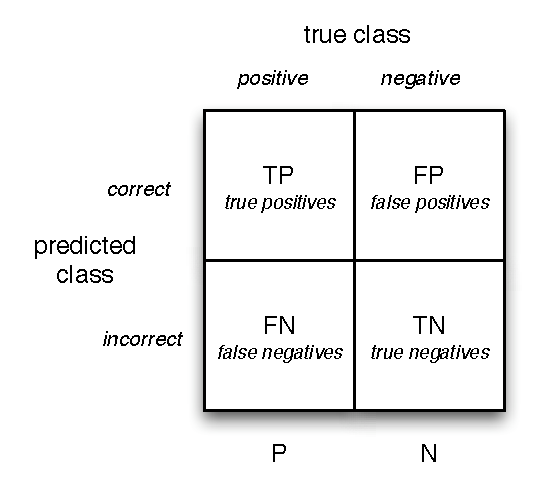
\epsfig{file=pos-neg.eps, width=0.5\textwidth}
\vspace*{-0.5cm}
\end{center}
\caption{Class-specific confusion matrix containing the basic counts
  used in the advanced performance metrics. \label{confmat}}
\end{figure}

Figure~\ref{confmat} displays the general confusion matrix\index{confusion matrix} for one class $C$, splitting all classifications on a test set into four cells. The TP or true positives cell contains a count of examples that have class $C$ and are predicted to have this class correctly by the classifier. The FP or false positives cell contains a count of examples of a different class that the classifier incorrectly classified as $C$. The FN or false negatives cell contains examples of class $C$ for which the classifier predicted a different class label than $C$.  On the basis of these four numbers and the total number of positive examples $P=TP+FN$ and negative examples $N=FP+TN$, we can compute the following performance measures:

\begin{description}
\item[Precision]\index{precision} $= \frac{TP}{TP+FP}$, or the
  proportional number of times the classifier has correctly made the
  decision that some instance has class $C$. 

\item[Recall or True Positive Rate
  (TPR)]\index{TPR}\index{recall}\index{true positive rate} $=
  \frac{TP}{P}$, or the proportional number of times an example with
  class $C$ in the test data has indeed been classified as class $C$
  by the classifier. 

\item[False Positive Rate (FPR)]\index{FPR}\index{false positive rate} $=
  \frac{FP}{N}$, or the proportional number of times an example with a
  different class than $C$ in the test data has been classified as
  class $C$ by the classifier.

\item[F-score]\index{F-score} $= \frac{2 \times precision \times
  recall}{precision + recall}$, or the harmonic mean\index{harmonic
  mean} of precision and recall \cite{VanRijsbergen79}, is a commonly
  used metric to summarize precision and recall in one measure. The
  left part of Figure~\ref{spaces} shows F-score isolines in the
  two-dimensional space of recall (x-axis) and precision (y-axis). The
  curvature of the isolines is caused by the harmonic aspect of the
  formula (in contrast, the normal mean has straight isolines
  orthogonal to the $x=y$ diagonal), which penalizes large differences
  between precision and recall. The isolines could be likened to
  height isolines in a map, where the peak of the hill is at the upper
  right corner of the space.

\item [AUC]\index{AUC}\index{area under the curve} or {\em area under
  the curve}\/ in the so-called ROC\index{ROC space} or {\em receiver
  operator characteristics}\/\index{receiver operator characteristics}
  space \cite{Egan75,Swets+00}, is the surface of the grey area in the
  right graph of Figure~\ref{spaces}. The ROC space is defined by the
  two dimensions FPR (false positive rate, x-axis) and TPR (true
  positive rate, or recall, y-axis). The difference with F-score is
  that it does not make use of the statistically unreliable precision
  metric; rather, it takes into account all cells of the matrix in
  Figure~\ref{confmat} including the TN (true negative) cell (for a
  more detailed description and arguments for using ROC analysis,
  cf. \cite{Fawcett04}). Its ``peak'' is in the upper left corner,
  at a FPR of zero and a TPR of 1. Rather than using the harmonic
  mean, it is common to report on the AUC, area under the classifier's
  TPR-FPR curve, where in the case of a discrete-output classifier
  such as {\sc TiMBL} this can be taken to mean the two lines
  connecting the experiment's TPR and FPR to the $(0,0)$ coordinate
  and the $(1,1)$ coordinate, respectively; the AUC is then the grey
  area between these points and coordinate $(1,0)$.

\end{description}

While these advanced statistics can be computed per class, they can also be averaged to produce a single outcome for a full test set. Common methods for averaging F-scores and AUC scores are micro-averaging and macro-averaging. In micro-averaging, each class' F-score or AUC is weighted proportionally to the frequency of the class in the test set. A macro-average adds all the F-scores or AUCs and divides this sum by the number of classes in the training set. In computing these averages, TiMBL bases itself on the classes in the training set. When a class does not re-occur in test material, it can have no recall, but it can have precision, hence it is always incorporated in averages. A class that occurs in test material but not in training material can never be predicted correctly, and is never included in averages.

\begin{figure}
\begin{center}

\begin{minipage}[t]{0.53\textwidth}
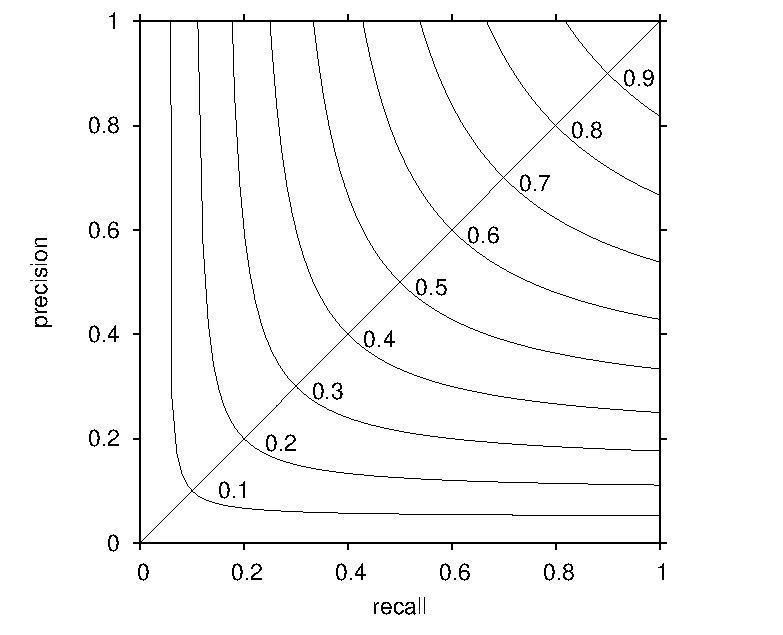
\epsfig{file=fspace.eps, width=\textwidth}
\end{minipage}\hfill
\begin{minipage}[t]{0.47\textwidth}
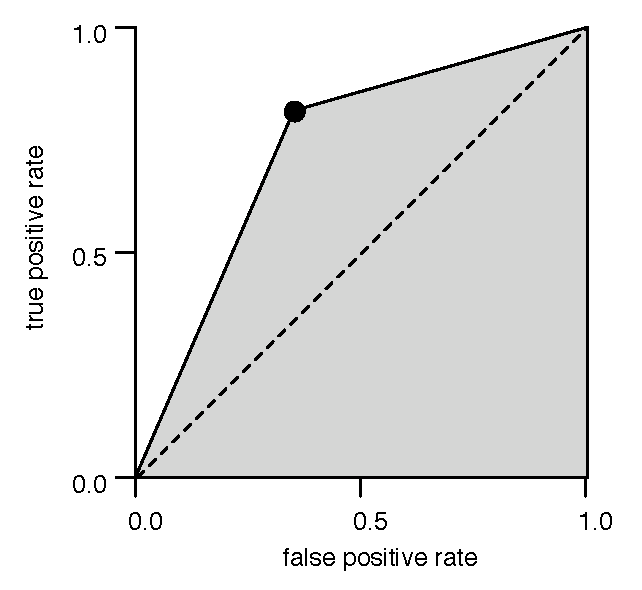
\epsfig{file=roc-auc.eps, width=\textwidth}
\end{minipage}

\end{center}
\caption{Precision--recall space with F-score isolines (left), and ROC
  space with an experimental outcome marked by the dot, and the
  outcome's AUC, the shaded surface between the dot and coordinates
  $(0,0)$, $(1,0)$, and $(1,1)$ (right). \label{spaces}}
\end{figure}



\section{NLP applications of TiMBL}
\label{furtherreading}

This section provides a brief historical overview of work, performed
in the Tilburg and Antwerp groups and by others, with the application
of {\sc mbl}-type algorithms to NLP tasks. For more historical
background, see \cite{Daelemans+05}.

The Tilburg and Antwerp groups have published a number of articles
containing descriptions of the algorithms and specialised metrics
collected in TiMBL, usually demonstrating their functioning using NLP
tasks. The {\sc ib1-ig} algorithm was first introduced in
\cite{Daelemans+92b} in the context of a comparison of memory-based
approaches with error-back\-propagation learning for a hyphenation
task.  Predecessor versions of {\sc igtree} can be found in
\cite{Daelemans+93c,VandenBosch+93} where they are applied to
grapheme-to-phoneme conversion.  See \cite{Daelemans+97} for a
description and review of {\sc igtree} and {\sc ib1-ig}. {\sc tribl}
is described in \cite{Daelemans+97d}.  Experiments with
distance-weighted class voting are described in
\cite{Zavrel97}. Aspects of using binary-valued (unpacked
multi-valued) features are discussed in \cite{VandenBosch+00}.
Comparisons between memory-based learning and editing variants are
reported in \cite{VandenBosch99,Daelemans+99}. A hybrid of TiMBL and
the {\sc ripper} rule-induction algorithm \cite{Cohen95} is described
in \cite{VandenBosch00,VandenBosch04}. Using TiMBL as a classifier
combination method is discussed in
\cite{Halteren+01}. \namecite{Raaijmakers00} describes an extension of
TiMBL with error-correcting output codes. \namecite{Hendrickx+04}
report on an experiment to import maximum-entropy matrices to replace
{\sc mvdm} matrices \cite{Hendrickx+04}, improving over the
maximum-entropy classifier. \namecite{VandenBosch04} presents a search
algorithm to find optimal combinations of parameter settings
automatically, given a labeled training set of examples, showing large
gains of the default settings (also of other machine learning
algorithms). Parallelization of TiMBL, through splitting either the
training set or the test set in $n$ pieces in shared-memory
multi-processor architectures, is explored in \cite{VandenBosch+07b}.

The memory-based algorithms implemented in the TiMBL package have been
targeted to a large range of Natural Language Processing
tasks. Examples of applications in the morpho-phonological and speech
areas are hyphenation and syllabification \cite{Daelemans+92b};
classifiying phonemes in speech \cite{Kocsor+00}; assignment of word
stress \cite{Daelemans+94}; grapheme-to-phoneme conversion,
\cite{VandenBosch+93,Daelemans+96,Canisius+06}; diminutive formation
\cite{Daelemans+98a}; and morphological analysis
\cite{VandenBosch+96,VandenBosch+99,Canisius+06}. Although these
examples are applied mostly to Germanic languages (English, Dutch, and
German), applications to other languages with more complicated writing
systems or morphologies, or with limited resources, have also been
presented: for example, letter-phoneme conversion in Scottish Gaelic
\cite{Wolters+97}, morphological analysis of Arabic \cite{Marsi+05},
or diacritic restoration in languages with a diacritic-rich writing
system \cite{Mihalcea02,DePauw+07}.

At the syntactic sentence level TiMBL has been applied to part of
speech tagging \cite{Daelemans+96b,Zavrel+99,Halteren+01};
PP-attachment \cite{Zavrel+97b}; subcategorization \cite{Buchholz98};
phrase chunking \cite{Veenstra98,Sang+99}; dependency parsing
\cite{Canisius+06b}, article generation \cite{Minnen+00}; shallow
parsing \cite{Daelemans+99a,Buchholz+99,Yeh00}; clause identification
\cite{Orasan00,Sang01}; sentence-boundary detection
\cite{Stevenson+00}; predicting the order of prenominal adjectives for
generation \cite{Malouf00}; and, beynd the sentence level, to anaphora
resolution \cite{Preiss02,Mitkov+02,Hoste05}. More recently,
memory-based learning has been integrated as a classifier engine in
more complicated dependency parsing systems
\cite{Nivre+04,Sagae+05,Canisius+06b}.

Memory-based learning has been applied succesfully to lexical
semantics, in particular to word sense disambiguation
\cite{Veenstra+00,Stevenson+99,Kokkinakis00,Mihalcea02,Hoste+02,DeCadt+04},
but also in other lexical semantic tasks such as determining noun
countability \cite{Baldwin+03}, animacy \cite{Orasan+01}, and semantic
relations within noun compounds \cite{Kim+06b,Nastase+06}.

On the textual level, TiMBL has been used for information extraction
\cite{Zavrel+00b,Zavrel+03,Ahn06}, text classification
\cite{Spitters00}, question classification \cite{Garcia+06,Dridan+07},
spam filtering \cite{Androutsopoulos+00}, named-entity recognition
\cite{Buchholz+00,Hendrickx+03,DeMeulder+03,Sporleder+06b,Leveling+06},
and error detection in textual databases \cite{Sporleder+06}.

In the field of discourse and dialogue modeling, TiMBL has been used
for shallow semantic analysis of speech-recognised utterances
\cite{Gustafson+99,Krahmer+01,VandenBosch+01,Lendvai+02a,Lendvai+03},
in disfluency detection in transcribed spontaneous speech
\cite{Lendvai+03c}, and in classifying ellipsis in dialogue
\cite{Fernandez+04}.

Relations to statistical language processing, in particular the
interesting equivalence relations with back-off smoothing in
probabilistic classifiers, are discussed in
\cite{Zavrel+97}. Relations between classification-based word
prediction and statistical language modeling are identified in
\cite{VandenBosch05,VandenBosch06}.

In machine translation, $k$-nearest neighbor classification bears a
close relation with example-based machine translation (EBMT). A first
EBMT-implementation using TiMBL is described in \cite{VandenBosch+07}.

The first dissertation-length study devoted to the approach is
\cite{VandenBosch97}, in which the approach is compared to alternative
learning methods for NLP tasks related to English word pronunciation
(stress assignment, syllabification, morphological analysis,
alignment, grapheme-to-phoneme conversion). TiMBL is also central in
the Ph.D. theses of \namecite{Buchholz02}, \namecite{Lendvai04},
\namecite{Hendrickx05} \namecite{Hoste05},
\namecite{Keuleers08}, and \namecite{Canisius09}. In 1999 a special issue of the {\em Journal for
  Experimental and Theoretical Artificial Intelligence} (Vol.~11(3),
edited by Walter Daelemans) was devoted to Memory-Based Language
Processing. The introduction to this special issue discusses the
inspiration sources and alternative developments related to the
memory-based approach taken in TiMBL \cite{Daelemans99b}.

Whereas most work using TiMBL has been oriented towards natural
language engineering applications, the linguistic and psycholinguistic
relevance of memory-based learning is another focus of research in
Antwerp, Tilburg and elsewhere. Work in this area has been done on
stress assignment in Dutch \cite{Daelemans+94,Gillis+00}, reading
aloud \cite{VandenBosch+00b}, phonological bootstrapping
\cite{Durieux+00}, the prediction of linking morphemes
in Dutch \cite{Krott+01}, morphology \cite{Eddington00,Eddington03},
and the Dutch plural inflection \cite{Keuleers+07}. A comparison to
other analogical methods for linguistics is provided in
\cite{Daelemans+97f,Daelemans02}.

\ \\

{\it All Tilburg/Antwerp papers referred to in this section, as well
as more recent papers, are available in electronic form from the {\sc
ILK} home page: {\tt http://ilk.uvt.nl} and the {\sc CLiPS} home page: \\
{\tt http://www.clips.ua.ac.be/}.}

\chapter{Software usage and options}
\label{reference}

\section{Command line options}
\label{commandline}

The user interacts with TiMBL through the use of command line arguments.
When you have installed TiMBL successfully, and you type {\tt Timbl} at the
command line without any further arguments, it will print an overview
of the most basic command line options. 

{\footnotesize
\begin{verbatim}
TiMBL 6.2.0 (c) ILK 1998 - 2009.
Tilburg Memory Based Learner
Induction of Linguistic Knowledge Research Group, Tilburg University
CLiPS Computational Linguistics Group, University of Antwerp
Mon Oct 19 22:33:13 2009

usage:  Timbl -f data-file {-t test-file}
or see: Timbl -h
        for all possible options
\end{verbatim}
}

If you are satisfied with all of the default settings, you can proceed
with just these basics:

\begin{description}

\item {\tt -f <datafile>} : supplies the name of the file with the
training items.
\item {\tt -t <testfile>} : supplies the name of the file with the
test items.
\item {\tt -h} : prints a glossary of all available command line 
options.

\end{description}

The presence of a training file will make TiMBL pass through the first two phases of its cycle. In the first phase it examines the contents of the training file, and computes a number of statistics on it (feature weights etc.). In the second phase the instances from the training file are stored in memory. If no test file is specified, the program exits, possibly writing some of the results of learning to files (see below). If there is a test file, the selected classifier, trained on the present training data, is applied to it, and the results are written to a file the name of which is a combination of the name of the test file and a code representing the chosen algorithm settings. TiMBL then reports the percentage of correctly classified test items. The default settings for the classification phase are: a Memory-Based Learner, with Gain Ratio feature weighting, with $k=1$, and with optimizations for speedy search. If you need to change the settings, because you want to use a different type of classifier, or because you need to make a trade-off between speed and memory-use, then you can use the options that are shown using {\tt -h}. The sections below provide a reference to the use of these command line arguments, and they are roughly ordered by the type of action that the option has effect on. Note that some options (listed with ``{\tt +/-}'') can be turned on ({\tt +}) or off ({\tt -}).

\subsection{Algorithm and metric selection}

\begin{description}

\item {\tt -a <n> or <string>} : determines the classification
algorithm. Possible values are:

	\begin{description}
	\item {\tt 0} or {\tt IB1} -- the {\sc ib1} ($k$-NN) algorithm (default). See Sections~\ref{mbl} and~\ref{indexing}.
	\item {\tt 1} or {\tt IGTREE} -- {\sc igtree}, decision-tree-based optimization. See Section~\ref{igtree}.
	\item {\tt 2} or {\tt TRIBL} -- {\sc tribl}, a hybrid of {\sc ib1} and {\sc igtree}. See Section~\ref{tribl}.
	\item {\tt 3} or {\tt IB2} -- {\sc ib2}, incremental edited memory-based learning. See Section~\ref{ib2}.
	\item {\tt 4} or {\tt TRIBL2} -- {\sc tribl2}, a non-parameteric version of {\sc tribl}. See Section~\ref{tribl}.
	\end{description}

\item {\tt -m <string>} : determines which distance metrics are used
for each feature. The format of this string is as follows:\\ {\tt
GlobalMetric:MetricRange:MetricRange}\\ Where {\tt GlobalMetric} is
used for alle features except for the ones that are assigned other
metrics by following the restrictions given by {\tt :MetricRange}.  A
range can be written using comma's for lists, and hyphens for
intervals. The metric code can be one of the following nine:

\begin{itemize}
\item {\tt O} -- Overlap (default; see Subsection~\ref{overlap})
\item {\tt M} -- Modified value difference ({\sc mvdm}; see Subsection~\ref{mvdm})
\item {\tt J} -- Jeffrey divergence (see Subsection~\ref{mvdm})
\item {\tt D} -- Dot product (see Subsection~\ref{dotproduct})
\item {\tt C} -- Cosine (see Subsection~\ref{dotproduct})
\item {\tt N} -- Numeric (all features are numeric. see Subsection~\ref{overlap})
\item {\tt L} -- Levenshtein (see Subsection~\ref{overlap})
\item {\tt DC} -- Dice coefficient (see Subsection~\ref{overlap})
\item {\tt I} -- Ignore (ignore specified features)
\end{itemize}

For example, {\tt -mO:N3:I2,5-7} sets the global metric to overlap,
declares the third feature to be numeric, and ignores features 2 and
5, 6, and 7.

Ignore {\em can}\/ be the global metric; it must be followed by a {\tt MetricRange} string with metric {\tt O}, {\tt M}, {\tt J}, {\tt D}, or {\tt N} specifying in the range which features are {\em not}\/ ignored.

\item {\tt -w <n>} : chooses between feature-weighting possibilities.
The weights are used in the metric of {\sc ib1} and in the ordering of the
{\sc igtree}. Possible values are:

	\begin{description}
	\item n=0 -- No weighting, i.e. all features have the same
	importance (weight = 1).
	\item n=1 -- Gain Ratio weighting (default). See section~\ref{infogain}.
	\item n=2 -- Information Gain weighting. See section~\ref{infogain}.
	\item n=3 -- Chi-squared ($\chi^2$) weighting. See section~\ref{chisquared}.
	\item n=4 -- Shared variance weighting. See section~\ref{chisquared}.
	\item n=$<$filename$>$:$<$number$>$ or n=$<$filename$>$ --
          Instead of the five weight settings above we can supply a
          filename to the {\tt -w} option. This causes TiMBL to read
          this file and use its contents as weights. If only
          $<$filename$>$ is given as an argument, the file is supposed
          to contain one list of feature weights for all features. The
          $<$filename$>$:$<$number$>$ option assumes that a weights
          file generated by TiMBL with the {\tt -W} option (and
          possibly edited by the user) is read back in; the number
          refers to one of the five numbers above. See
          section~\ref{weightformat} for a description of the format
          of weights files.
	\end{description}

\item {\tt -k <n>} : number of nearest neighbors used for
        extrapolation. Only applicable in conjunction with {\sc ib1}
        ({\tt -a 0}), {\sc tribl} ({\tt -a 2}), {\sc tribl2} ({\tt -a
          4}) and {\sc ib2} ({\tt -a 3}). The default is 1. Especially
        with the {\sc mvdm} metric it is often useful to determine a
        good value larger than 1 for this parameter (usually an odd
        number, to avoid ties). Note that due to ties (instances with
        exactly the same similarity to the test instance) the number
        of instances used to extrapolate might in fact be much larger
        than this parameter.

\item {\tt -d <val>} : The type of class voting weights that are used for
extrapolation from the nearest neighbor set. {\tt val} can be one of:
	\begin{itemize} 

  	\item {\tt Z} : normal majority voting; all neighbors have
         equal weight (default).

  	\item {\tt ID}: Inverse Distance weighting. See
  	Section~\ref{distweightvote}, Equation~\ref{dudani_eq}.

  	\item {\tt IL}: Inverse Linear weighting. See
  	Section~\ref{distweightvote}, Equation~\ref{inverseweight}.

  	\item {\tt ED:<a>:<b>}: Exponential Decay weighting with decay
  	parameters {\tt a} ($\alpha$) and {\tt b} ($\beta$). No spaces
  	are allowed in the string. Parameter {\tt b} can be left
  	unspecified: {\tt ED:<a>} assumes $\beta=1$. The syntax used
  	in previous TiMBL versions ({\tt ED<a>}) is still supported
  	but deprecated. See Section~\ref{distweightvote},
  	Equation~\ref{expdecayweight}.

\end{itemize}

\item {\tt -L <n>} : frequency threshold for switching from the {\sc
    mvdm} or Jeffrey Divergence to the Overlap distance metric. The
  default is 1 (never switch). When in a pair of matched values one or
  both values occur less frequently than {\tt n} times in the learning
  material, TiMBL switches from {\sc mvdm} or Jeffrey Divergence to
  Overlap. Higher values of {\tt n} force TiMBL to use the Overlap
  metric more. 

 Only applicable in conjunction with the {\sc mvdm}
  ({\tt -mM}) and Jeffrey divergence ({\tt -mJ}) distance metrics.


\item {\tt -b <n>} : determines n ($\geq 1$), the number of instances,
to be taken from the top of the training file, to act as the bootstrap
set of memorized instances before {\sc ib2} starts adding new
instances. Only applicable in conjunction with {\sc ib2} ({\tt -a 3}).

\item {\tt -q <n>} : {\tt n} is the {\sc tribl} offset, the index
number of the feature (counting from 1) after which {\sc tribl} should
switch from {\sc igtree} to {\sc ib1}. Only applicable in conjunction
with {\sc tribl} ({\tt -a 2}).

\item {\tt -R <n>} : Resolve ties in the classifier randomly, using a
random generator with seed n. {\tt -R <n>} causes the classification
to be based on a random pick (with seed n) of a category according to
the probability distribution in the nearest neighbor set. By default,
{\tt -R} is not used, but rather the deterministic tie resolution
scheme described in Subsection~\ref{overlap}.

\item {\tt -t $<$@file$>$} : If the filename given after {\tt -t} starts
with '{\tt @}', TiMBL will read commands for testing from {\tt file}.
This file should contain one set of instructions per line. On each
line new values can be set for the following command line options:
{\tt -B -d -e -k -L -M -o -p -Q -R -t -u +/-v -w +/-x +/-\%}. It is
compulsory that each line in {\tt file} contains a {\tt -t <testfile>}
argument to specify the name of the test file.

\item {\tt -t <testfile>} : the string {\tt <testfile>} is the literal name
of the file with the test items.

\item {\tt -t leave\_one\_out} : No test file is read, but testing is
done on each pattern of the training file, by treating each pattern of
the training file in turn as a test case (and the whole remainder of
the file as training cases). Only applicable in conjunction with {\sc ib1} ({\tt -a0}).

\item {\tt -t cross\_validate} : An $n$-fold cross-validation
experiment is performed on the basis of $n$ files (e.g. $1/n$
partitionings of an original data file). The names of these $n$ files
need to be in a text file (one name per line) which is given as
argument of {\tt -f}. In each fold $f=1 \ldots n$, file number $f$ is
taken as test set, and the remaining $n-1$ files are concatenated to
form the training set. Only applicable in conjunction with {\sc ib1} ({\tt -a0}).

\end{description}

\subsection{Input options}

\begin{description}

\item {\tt -f <datafile>} : the string {\tt <datafile>} is the literal
name of the file with the training items, or (in conjunction with {\tt
-t cross\_validate}, the file containing the names of the
cross-validation files.

\item {\tt -F <format>} : Force TiMBL to interpret the training and
test file as a specific data format. Possible values for this
parameter are: {\tt Compact, C4.5, ARFF, Columns, Sparse, Binary}
(case-insensitive). The default is that TiMBL guesses the format from
the contents of the first line of the data file. ARFF is not
automatically detected. See section~\ref{dataformats} for description
of the data formats and the guessing rules. The {\tt Compact} format
cannot be used with numeric features.

\item {\tt -l <n>} : Feature length. Only applicable with the Compact
  data format; {\tt <n>} is the number of characters used for each
  feature-value and category symbol.

\item {\tt -i <treefile>} : Skip the first two training phases:
  instead of processing a training file, read a previously saved (see
  {\tt -I} option) instance-base or {\sc igtree} from the file {\tt
    treefile}. See section~\ref{treeformat} for the format of this
  file.

\item {\tt --matrixin=<filename>} : Read value distance metrics (such as {\sc mvdm} or Jeffrey divergence matrices written to file with {\tt --matrixout=<filename}, or from user-generated matrices) from file {\tt filename}.

\item {\tt -u <valueclassprobfile>} : Replace the automatically
  computed value-class probability matrix with the matrices provided
  in this file.

\item {\tt -P <path>} : Specify a path to read the data files
  from. This path is ignored if the name of the data file already
  contains path information.

\item {\tt -s}: Use the whitespace-delimited exemplar weights, given
  after each training instance in the training file {\tt <datafile>},
  during classification. {\tt <testfile>} may contain exemplar
  weights, but they are not used in classification. If the test file
  does not have an exemplar weights column, you must specify {\tt
    -s1}. Exemplar weights can also be ignored (in both training and
  test files) by specifying {\tt -s0}.

\end{description}

\subsection{Output options}

\begin{description}

\item {\tt -I <treefile>} : After phase two of learning, save
  the resulting tree-based representation of the instance-base or {\sc
    igtree} in a file. This file can later be read back in using the
  {\tt -i} option (see above). For {\sc igtree} this also automatically
  saves the current weights into {\tt treefile.wgt} unless this is
  overridden by {\tt -W}.
  See section~\ref{treeformat} for a description of the resulting file's format.

\item {\tt --matrixout=<filename>} : Store calculated {\sc mvdm} or Jeffrey divergence distance metrics in file {\tt filename}.

\item {\tt -X <xmlfile>} : instead of the proprietary file format
  written with the {\tt -I} switch, {\tt -X} writes the TiMBL tree
  into an XML tree in {\tt <xmlfile>}. This XML file cannot be read
  back into TiMBL.

\item {\tt -W <file>} : Save the currently used feature-weights in a
file.

\item {\tt -U <valueclassprobfile>} : Write the automatically computed
value-class probability matrix to this file.

\item {\tt -n <file>} : Save the feature-value and target category
symbols in a C4.5 style ``names file'' with the name {\tt
<file>}. Take caution of the fact that TiMBL does not mind creating a
file with ',' '.' '$|$' and ':' values in features; C4.5 will produce errors on this.

\item {\tt -p <n>} : Indicate progress during training and testing
after every n processed patterns. The default setting is 100,000.

\item {\tt -e <n>} : During testing, compute and print an estimate on
how long it will take to classify n test patterns. Off by
default.

\item {\tt +/-v <n>} : Verbosity Level; determines how much
information is written to the output during a run. Unless indicated
otherwise, this information is written to standard error. The use of
{\tt +} turns a given verbosity level {\bf on}, whereas {\tt -} turns
it {\bf off} (only useable in non-commandline contexts, such as
client/server communication or {\tt -t @testcommandfile}). This
parameter can take on the following values (case-insensitive):

	\begin{description}
         \item {\tt s}:  work silently (turns off all set verbosity levels).
         \item {\tt o}:  show all options set.
         \item {\tt f}:  show calculated feature weights. (default)
         \item {\tt p}:  show {\sc mvdm} matrices.
         \item {\tt e}:  show exact matches.
         \item {\tt as}: show overall advanced statistics (micro and macro averages of F-score and AUC).
	 \item {\tt cm}: show confusion matrix between actual and predicted classes.
         \item {\tt cs}: show per-class statistics (precision, recall, true positive rate, false positive rate, F-score, AUC).
         \item {\tt di}: add the distance of the nearest neighbor to the output file.
         \item {\tt db}: add class distribution in the nearest neighbor set to the output file.
         \item {\tt md}: add matching depth and node type (N for non-ending
           node, L for leaf) to output file.
	 \item {\tt k}:  add a summary of class distribution information of all nearest neighbors to the output file (sets {\tt -x})
         \item {\tt n}:  add nearest neigbors to the output file (sets {\tt -x})
         \item {\tt b}:  provide branching statistics of the internal tree, overall and per level.
	\end{description}

        You may combine levels using '{\tt +}' e.g. {\tt +v p+db} or
        {\tt -v o+di}.

\item {\tt -G <n>}: Normalize class distributions generated by {\tt +v db}.
  \begin{description}
    \item {\tt 0 (zero)}: Normalize distributions so that they add up to 1.0
    \item {\tt 1:<f>}: Smooth by adding floating-point $f$ to all class votes (e.g. {\tt -G1:1} performs add-one smoothing).
  \end{description}

\item {\tt --Beam=<n>}: Limit the number of returned classes and class
  votes returned by {\tt +v db} to $n$. Default is infinity (no limit).

\item {\tt +/- \%} : Write the percentage of correctly classified test
  instances, the number of correctly classified instances, and the
  total number of classified instances (one number per line, three
  lines in total) to a file with the same name as the output file, but
  with the suffix ``{\tt .\%}''.

\item {\tt -o $<$filename$>$} : Write the test output to filename. Useful
  for different runs with the same settings on the same testfile,
  where the default output file name would normally be the same.

\item {\tt -O $<$path$>$} : Write all output to the path given here. The
  default is to write all output to the directory where the test file
  is located.

\item {\tt -V} : Show the TiMBL version number.

\end{description}

\subsection{Internal representation options}

\begin{description}

\item {\tt -N <n>} : (maximum) number of features. Obligatory for
  Sparse and Binary formats. When larger than a pre-defined constant
  (default 2500), N needs to be set explicitly for all algorithms.

\item {\tt +/- x} : turns the shortcut search for exact matches on or
  off in {\sc ib1} (and {\sc ib2}, {\sc tribl}, and {\sc tribl2}). The
  default is to be off ({\tt -x}). Turning it on makes {\sc ib1}
  generally faster, but with $k>1$ the shortcut produces different
  results from a genuine $k$ nearest neighbors search, since absolute
  preference is given to the exact match.

\item {\tt -M <n>} : Set the maximum number of nearest neighbors
  printed using the {\tt +vn} verbosity option. By default this is set
  to 500, but when you are interested in the contents of really large
  nearest neighbor sets (which is possible with large $k$ or large
  data sets with few features), {\tt n} can be increased up to
  100,000.

\item {\tt +/- H} : Turn on/off hashing of feature values and class
  labels in TiMBL trees. Hashing is done by default, but with short
  (e.g. one-character) feature values and/or classes less memory is
  used when hashing is set off.

\item {\tt -B <n>} : Number of bins used for discretizing numeric data
  (only used for computing feature weights).

\item {\tt -c <n>} : Clipping (threshold) frequency for prestoring
  {\sc mvdm} matrices. Cells in the matrix are only stored if both
  feature values occur more than {\tt <n>} times.

\item {\tt -T <string>} : Set the ordering of the TiMBL tree (with
  {\sc ib1} and {\sc ib2}), i.e., rank the features according to the
  metric identified by {\tt <string>}. The default ordering is {\tt
    G/V} (according to gain ratio divided by the number of values),
  but some orderings may produce faster classification. Note that
  different orderings do {\em not}\/ change the classification
  behavior of {\sc ib1} and {\sc ib2}. {\tt <string>} can take the
  following values:

	\begin{description}
         \item {\tt DO}: no ordering (the ordering of the features in
           the data file is taken)
         \item {\tt GRO}: gain ratio (eq.~\ref{IGgainratio})
         \item {\tt IGO}: information gain (eq.~\ref{IGgain})
         \item {\tt 1/V}: $1/V$, where $V$ is the number of values
         \item {\tt G/V}: gain ratio divided by the number of values
         \item {\tt I/V}: information gain divided by the number of
           values
         \item {\tt X2O}: \chisq \ (eq.~\ref{chisq-eq})
         \item {\tt X/V}: \chisq \ divided by the number of values
         \item {\tt SVO}: shared variance
           (eq.~\ref{shared-variance-eq})
         \item {\tt S/V}: shared variance divided by the number of
           values
         \item {\tt GxE}: gain ratio $\times si$, where $si$ is the
           split info of the feature (eq.~\ref{splitinfo})
         \item {\tt IxE}: information gain $\times si$
         \item {\tt 1/S}: $1/si$
	\end{description}

\end{description}

\subsection{Hidden options}

TiMBL offers an undisclosed number of hidden options that have been built in over time for particular reasons. Some have survived over time, and although their use is not for the faint-hearted, some may offer interesting functionalities. A small list of disclosed hidden options follows.

\begin{description}
  \item {\tt --sloppy=\{true|false\}}: in combination with leave-one-out (LOO) testing, this option turns off all weight recomputation. By default, leaving out one training example out causes all feature weights, value-class matrices, and derived metrics such as {\sc mvdm} to be recomputed, because strictly the example-specific statistics should be absent when it is held out and classified. {\tt --sloppy} skips this, causing a significant speedup, and usually slightly better LOO scores. Use only if your experimental method allows it. Default value is {\tt false}.
  \item {\tt --silly=\{true|false\}}: set to {\tt true}, switches off the optimized nearest-neighbor search in {\sc ib1} and {\sc tribl}. This causes TiMBL to fall back to comparing all feature values of a test instance to full paths in the TiMBL tree. This causes TiMBL to slow down dramatically on most datasets. Setting is available to enable testing the effect of optimized search. Default value is {\tt false}.
  \item{\tt --Diversify}: modifies all features weights by subtracting the smallest weight (plus $\epsilon$) from all weights. The smallest weight thus becomes $\epsilon$. This modification ``diversifies'' the feature weights, and was introduced to enhance the effect of {\sc Dimbl}, the multi-CPU variant of TiMBL\footnote{For {\sc Dimbl}, see \url{http://ilk.uvt.nl/dimbl}}.
\end{description}

\section{File formats}
\label{fileformats}

This section describes the format of the input and output files used
by TiMBL. Where possible, the format is illustrated using the
classical ``objects'' data set, which consists of 12 instances of 5
different everyday objects (nut, screw, key, pen, scissors), described
by 3 discrete features (size, shape, and number of holes).

\subsection{Data files}
\label{dataformats}

The training and test sets for the learner consist of descriptions of
instances in terms of a fixed number of feature-values. TiMBL supports
a number of different formats for the instances, but they all have in
common that the files should contain one instance per line. The number
of instances is determined automatically, and the format of each
instance is inferred from the format of the first line in the training
set. The last feature of the instance is assumed to be the target
category. Should the guess of the format by TiMBL turn out to be
wrong, you can force it to interpret the data as a particular format
by using the {\tt -F} option. Note that TiMBL, by default, will
interpret features as having {\em symbolic, discrete values}. Unless
you specify explicitly that certain features are numeric, using the
{\tt -m} option, TiMBL will interpret numbers as just another string
of characters. If a feature is numeric, its values will be scaled to
the interval [0,1] for purposes of distance computation (see
Equation~\ref{overlapeq}). The computation of feature weights will be
based on a discretization of the feature.

Once TiMBL has determined the input format, it will skip and complain
about all lines in the input which do not respect this format
(e.g.~have a different number of feature-values with respect to that
format).

During testing, TiMBL writes the classifications of the test set to an
output file. The format of this output file is by default the same as
the input format, with the addition of the predicted category being
appended after the correct category. If we turn on higher levels of
verbosity, the output files will also contain distributions, distances
and nearest neighbor sets.

\subsubsection{Column format}
\label{comlumnformat}

The {\bf column format} uses white space as the separator between
features. White space is defined as a sequence of one or more spaces or
tab characters. Every instance of white space is interpreted as a
feature separator, so it is not possible to have feature-values
containing white space. The column format is auto-detected when an
instance of white space is detected on the first line {\em before a
comma has been encountered}. The example data set looks like this in
the column format:

\begin{footnotesize}
\begin{verbatim}
small	compact	1	nut
small	long	none	screw
small	long	1	key
small	compact	1	nut
large	long	1	key
small	compact	none	screw
small	compact	1	nut
large	long	none	pen
large	long	2	scissors
large	long	1	pen
large	other	2	scissors
small	other	2	key
\end{verbatim}
\end{footnotesize}

\subsubsection{C4.5 format}
\label{c45format}

This format is a derivative of the format that is used by the
well-known C4.5 decision tree learning program~\cite{Quinlan93}.  The
separator between the features is a comma, and the category (viz.  the
last feature on the line) is followed by a period (although this is
not mandatory: TiMBL is robust to missing periods)\footnote{The
periods after the category are not reproduced in the output}.  White
space within the line is taken literally, so the pattern {\tt a,\ b\
c,d} will be interpreted as {\tt `a',`\ b\ c',`d'}. An exception is the 
class label, which should not contain any whitespace. When using this
format, especially with linguistic data sets or with data sets
containing floating point numbers, one should take special care that
commas do not occur as feature values and that periods do not
occur within the category.  Note that TiMBL's C4.5 format does not
require a so called {\em namesfile}.  However, TiMBL can produce such
a file for C4.5 with the {\tt -n} option.  The C4.5 format is
auto-detected when a comma is detected on the first line {\em before
any white space has been encountered}. The example data set looks like
this in the C4.5 format:

\begin{footnotesize}
\begin{verbatim}
small,compact,1,nut.
small,long,none,screw.
small,long,1,key.
small,compact,1,nut.
large,long,1,key.
small,compact,none,screw.
small,compact,1,nut.
large,long,none,pen.
large,long,2,scissors.
large,long,1,pen.
large,other,2,scissors.
small,other,2,key.
\end{verbatim}
\end{footnotesize}

\subsubsection{ARFF format}
\label{arffformat}

ARFF is a format that is used by the WEKA machine learning
workbench~\cite{Garner95,Witten+99}\footnote{WEKA is available from
the Waikato University Department of Computer Science, \url{http://www.cs.waikato.ac.nz/~ml/weka}}.  Although TiMBL at present
does {\em not}\/ entirely follow the ARFF specification, it still
tries to do as well as it can in reading this format. The ARFF format
is {\em not}\/ autodetected, and needs to be specified on the
commanline with {\tt -F ARFF}.


In ARFF data, the actual data are preceded by a information on feature
types, feature names, and names of values in case of symbolic
features. TiMBL ignores all of these lines, and starts reading data
from after the {\tt @data} statement until the end of the
file. Feature-values are supposed to be separated by commas; white
space is deleted entirely, so the pattern {\tt a, b c,d} will be
interpreted as {\tt `a',`bc',`d'}. There should be no whitespace in
class labels.  We hope to include better support for the ARFF format
in future releases.

\begin{footnotesize}
\begin{verbatim}
% There are 4 attributes.
% There are 12 instances.
% Attribute information:                       Ints Reals  Enum  Miss
%          'size'                                 0     0    12     0   
%          'shape'                                0     0    12     0   
%          'n_holes'                              9     0     3     0   
%          'class.'                               0     0    12     0   
@relation 'example.data'
@attribute 'size' { small, large}
@attribute 'shape' { compact, long, other}
@attribute 'n_holes' { 1, none, 2}
@attribute 'class.' { nut., screw., key., pen., scissors.}
@data
small,compact,1,nut.
small,long,none,screw.
small,long,1,key.
small,compact,1,nut.
large,long,1,key.
small,compact,none,screw.
small,compact,1,nut.
large,long,none,pen.
large,long,2,scissors.
large,long,1,pen.
large,other,2,scissors.
small,other,2,key.
\end{verbatim}
\end{footnotesize}

\subsubsection{Compact format}
\label{compactformat}

The compact format is especially useful when dealing with very large
data files. Because this format does not use any feature separators,
file-size is reduced considerably in some cases. The price of this is
that all features and class labels must be of equal length (in
characters) and TiMBL needs to know beforehand what this length
is. You must tell TiMBL by using the {\tt -l} option. The compact
format is auto-detected when neither of the other formats applies. The
same example data set might look like this in the column format (with
two characters per feature):

\begin{footnotesize}
\begin{verbatim}
smco1_nu
smlonosc
smlo1_ke
smco1_nu
lalo1_ke
smconosc
smco1_nu
lalonope
lalo2_sc
lalo1_pe
laot2_sc
smot2_ke
\end{verbatim}
\end{footnotesize}

\subsubsection{Sparse format}

The sparse format is relevant for data with features of which a
significant portion of the values is $0.0$ (numeric), $0$ (binary), or
some ``null'' symbolic value. Storing only the non-null values
typically takes less space on disk.

Consider, for example, a data set in text classification with 10,000
features each representing the tf*idf weight of a term. It would be
uneconomical to store instances as long lines of

\begin{footnotesize}
\begin{verbatim}
0.02, 0.0, 0.0, 0.0, 0.54, 0.0, 0.0, 0.0, 0.0, 0.0, 0.0, 0.0, ... , 0.01,sports
\end{verbatim}
\end{footnotesize}

The Sparse format allows to store such an instance as

\begin{footnotesize}
\begin{verbatim}
(1,0.02)(5,0.54)...(10000,0.01)sports
\end{verbatim}
\end{footnotesize}

That is, a sequence of ($<index>,<value>$) expressions between
parentheses each indicating that the feature number $index$ has value
$value$, with the class label at the end, directly following the last
parenthesis. The feature index is assumed to start at 1. In case of
symbolic values, whitespace included in the parentheses are considered
significant (i.e., part of the values). A case with only null values
can be represented as either `{\tt class} or {\tt ,class}.

This option must be specified by the user ({\tt -F Sparse}); it is not
guessed from the data. It must also be accompanied by a user
declaration of the number of features ({\tt -N <number>}).

\subsubsection{Sparse Binary format}
\label{binaryformat}

The sparse binary format, a simplified version of the Sparse format,
is especially useful when dealing with large numbers of two-valued
(binary) features, of which each case only has a very few active ones,
such as e.g. in text categorization. Thus instead of representing a
case as:

\begin{footnotesize}
\begin{verbatim}
1,0,0,0,0,0,0,1,0,0,1,1,0,0,0,0,0,1,small.
\end{verbatim}
\end{footnotesize}

We can represent it as:

\begin{footnotesize}
\begin{verbatim}
1,8,11,12,18,small.
\end{verbatim}
\end{footnotesize}

This format allows one to specify only the index numbers of the active
features (indexes start at one), while implicitly assuming that the
value for all the remaining features is zero. Because each case has a
different number of active features, we must specify in some other way
what the actual number of features is. This must be done using the
{\tt -N} option.  As the format is very similar to numeric features,
it must always be user-declared using {\tt -F Binary}. The last
feature of a line is always interpreted as being the category
string. A case with only zeroes can be represented as either `{\tt
class} or {\tt ,class}.

\subsection{Weight files}
\label{weightformat}

The feature weights used for computing similarities and for the
internal organization of the memory base can be saved to a file {\tt
  -W}. These files can be read back into TiMBL with {\tt -w
  $<$filename$>$:$<$weight number$>$}, where the weight number refers to the
five options in TiMBL. It is also possible to change these files
manually before reading them in -- and additionally it is also
possible to write a file from scratch and read this into TiMBL. This
allows the experimenter to handcraft feature weights.

The generic format for the weights file is as follows.  The weights
file may contain comments on lines that start with a \# character. The
other lines contain the number of the feature followed by its numeric
weight. An example of such a file is provided below. The numbering of
the weights starts with 1. In this example, the data set has three features.

\begin{footnotesize}
\begin{verbatim}
# DB Entropy: 2.29248
# Classes: 5
# Lines of data: 12
# Fea.  Weight
1       0.765709
2       0.614222
3       0.73584
\end{verbatim}
\end{footnotesize}

Weight files written by TiMBL are of the same format, but write all
weights in a concatenation, separated by \# lines that carry the
abbreviated name of the weight (nw, gr, ig, x2, sv). The following
example illustrates this format (which can be edited manually, as long
as the same number of lines is kept):

\begin{footnotesize}
\begin{verbatim}
# DB Entropy: 1.61789
# Classes: 5
# Lines of data: 2999
# nw
# Fea.  Weight
1       1
2       1
3       1
#
# gr
# Fea.  Weight
1       0.0428445870345557
2       0.185070180760327
3       0.325371814230901
#
# ig
# Fea.  Weight
1       0.213887591411729
2       0.669704582861074
3       1.27807624584789
#
# sv
# Fea.  Weight
1       0.0762436694064095
2       0.233998145488354
3       0.596896311429044
#
# x2
# Fea.  Weight
1       914.619058199289
2       2807.0417532783
3       7160.36815190281
#

\end{verbatim}
\end{footnotesize}


\subsection{Value difference files}
\label{mvdmformat}

Using the {\sc mvdm} metric, it can sometimes be interesting to
inspect the matrix of conditional class probabilities from
Equation~\ref{MVDMeq}. By using the {\tt -U} option, we can write the
computed matrix to a file. This way we can see which values are
considered to be similar by the metric. For each feature a row vector
is given for each value, of the conditional probabilities of all the
classes (columns) given that value.

\begin{footnotesize}
\begin{verbatim}
targets A,      B,      C,      D,      E.

feature # 1 Matrix: 
small   0.429   0.286   0.286   0.000   0.000
large   0.000   0.000   0.200   0.400   0.400
 
feature # 2 Matrix: 
compact 0.750   0.250   0.000   0.000   0.000
long    0.000   0.167   0.333   0.333   0.167
other   0.000   0.000   0.500   0.000   0.500
 
feature # 3 Matrix: 
1       0.500   0.000   0.333   0.167   0.000
none    0.000   0.667   0.000   0.333   0.000
2       0.000   0.000   0.333   0.000   0.667
\end{verbatim}
\end{footnotesize}

As long as this format is observed, the file can be modified (manually
or by substituting some other vector-based representations for the
values), and the new matrix can be read in and used with the {\sc
mvdm} metric.

\subsection{Tree files}
\label{treeformat}

Although the learning phase in TiMBL is relatively fast, it can be useful to store the internal representation of the data set both for later usage and for faster subsequent learning. In TiMBL, the data set is stored internally in a tree structure (see Section~\ref{indexing}). When using {\sc ib1}, this tree representation contains all the training cases as full paths in the tree. When using {\sc igtree}, unambiguous paths in the tree are pruned before it is used for classification or written to file; on the same data, {\sc igtree} trees are usually considerably smaller than {\sc ib1} trees. In either tree type, the arcs represent feature values and nodes contain class distribution information. The features are in the same order throughout the tree. This order is either determined by memory-size considerations in {\sc ib1}, or by feature relevance in {\sc igtree}. It can explicitly be manipulated using the {\tt -T} option.

We strongly advise to refrain from manually editing the tree file. However, the syntax of the tree file is as follows. First a header consisting of information about the status of the tree, the feature-ordering (the permutation from the order in the data file to the order in the tree), and the presence of numeric features is provided\footnote{Although in this header each line starts with '\#', these lines cannot be seen as comment lines.}. Subsequently, unless hashing has been set off explicitly ({\tt -H}), a legenda is given of numeric hash codes for the class names (one unique integer per class) and feature value names (one unique integer per value).  Subsequently, the tree's nodes and arcs are given in a proprietary non-indented bracket notation.

Starting from the root node, each node is denoted by an opening parenthesis ``('', followed by an integer coding the default class. After this, there is the class distribution list, within curly braces ``\{ \}'', containing a non-empty list of category codes followed by integer counts. After this comes an optional comma-separated list of arcs to child nodes, within ``[ ]'' brackets. An arc is labeled with a coded feature value. The node that the arc leads to again has a class distribution, and any number of child nodes pointed to by arcs.

The {\sc ib1} tree constructed from our example data set looks as follows:

\begin{footnotesize}
\begin{verbatim}
# Status: complete
# Permutation: < 1, 3, 2 >
# Numeric: .
# Version 4 (Hashed)
#
Classes
1       nut
2       screw
3       key
4       pen
5       scissors
Features
1       small
2       compact
3       1
4       long
5       none
6       large
7       2
8       other

(1{ 1 3, 2 2, 3 3, 4 2, 5 2 }[1(1[3(1[2(1{ 1 3 })
,4(3{ 3 1 })
]
)
,5(2[2(2{ 2 1 })
,4(2{ 2 1 })
]
)
,7(3[8(3{ 3 1 })
]
)
]
)
,6(4[3(3[4(3{ 3 1, 4 1 })
]
)
,5(4[4(4{ 4 1 })
]
)
,7(5[4(5{ 5 1 })
,8(5{ 5 1 })
]
)
]
)
]
)

\end{verbatim}
\end{footnotesize}

The corresponding compressed {\sc igtree} version is considerably smaller. 

\begin{footnotesize}
\begin{verbatim}
# Status: pruned
# Permutation: < 1, 3, 2 >
# Numeric: .
# Version 4 (Hashed)
#
Classes
1       nut
2       screw
3       key
4       pen
5       scissors
Features
1       small
2       compact
3       1
4       long
5       none
6       large
7       2
8       other

(1{ 1 3, 2 2, 3 3, 4 2, 5 2 }[1(1{ 1 3, 2 2, 3 2 }[3(1{ 1 3, 3 1 }[4(3{ 3 1 })
]
)
,5(2{ 2 2 })
,7(3{ 3 1 })
]
)
,6(4{ 3 1, 4 2, 5 2 }[3(3{ 3 1, 4 1 })
,7(5{ 5 2 })
]
)
]
)

\end{verbatim}
\end{footnotesize}

TiMBL tree files generated by versions 1.0 to 3.0 of TiMBL, which do not contain hashed class and value names, are no longer recognized in current TiMBL versions. Backward compatibility to trees generated by versions 1.0 to 3.0 is preserved in TiMBL version 4 up to release 4.3.1.

\clearpage

\bibliographystyle{fullname}
\bibliography{ilk}

\end{document}
